\chapter{高輝度LHC-ATLAS実験に向けたエンドキャップミューオントリガーの統合}
\label{chap_TriggerIntegration}
高輝度LHC-ATLAS実験において、エンドキャップ部トリガーロジックは大規模論理回路としてSL FPGA上に実装される。トリガーロジックはこれまで、東京大学、京都大学、名古屋大学をはじめとするATLAS TGC JAPAN グループの共同研究として開発が進められてきた。本章ではまず、トリガーロジック開発の流れを説明する。次にこれまでに開発されたトリガーロジックのコンセプトとHDL実装について述べた後、本研究で行なった統合作業について述べる。

\section{トリガーロジック開発の流れ}
\label{sec_TriggerTestSystem}
本節では、高輝度LHC-ATLAS実験に向けたエンドキャップ部ミューオントリガー回路の開発流れを説明し、トリガー開発全体の流れにおける本研究の位置づけを説明する。図\ref{Trigger_flow}にトリガーロジックの開発フローを示す。トリガーロジックは最終的にバックエンドエレクトロニクスであるSLのFPGA上でデジタル回路として稼働するが、それまでにコンセプトの設計、モジュールごとのHDL実装、全体ファームウェアへの統合という3ステップで開発が進められてきた。また、それぞれの工程において検証システムも同時に構築することで、期待した性能をもつトリガーロジックが実現できていることを確かめながら、着実に開発が進められている。

\begin{figure} 
\centering
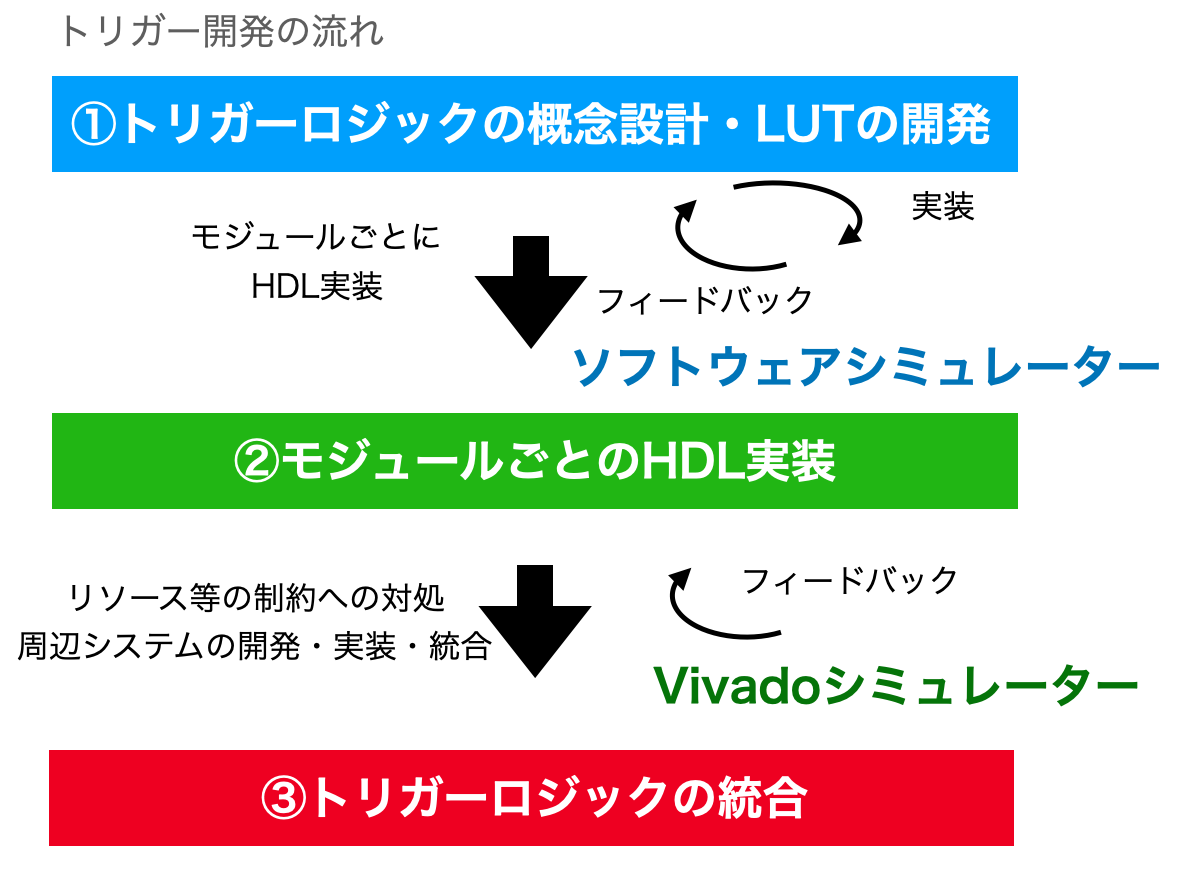
\includegraphics[width=16cm]{fig/SL/Trigger_flow.png}
\caption[TGCトリガー開発の流れ]{TGCトリガー開発の流れ。}
\label{Trigger_flow}
\end{figure}

\subsection*{トリガーロジックの概念設計}
トリガーの開発は、まず高輝度LHC-ATLAS実験におけるL0 Trigger systemの要求を満たすよう、概念的な設計を行う。L0 Trigger systemの要求には具体的にトリガー効率、再構成した角度分解能、トリガーレート、トリガーレイテンシーなどが含まれる。Run3ロジックの例でいうと、SLBでM1、M3間のコインシデンスをとり、HPTで3ステーションのコインシデンスをとり、SLでWireとStripのコインシデンスをとる、というようなグローバルな設計から、複数なヒットがあった場合にどのような優先順位で飛跡候補を選ぶか、という具体的な設計までこの段階で行われる。

設計されたロジックを、より具体的なデザインに落とし込み、性能を評価していく作業にはソフトウェアシミュレーターを用いる。ソフトウェアは開発が容易で、ロジックの実装→性能評価→ロジックの修正→…という開発サイクルを素早く回すことができる。そのため、グローバルなデザインを決めていく初期の開発には有用である。さらに、パターンマッチングに利用されるLUTもロジックの設計と同時にソフトウェア的に開発される。

\subsection*{モジュールごとのHDL実装}
コンセプト設計が固まったあとには、そのロジックを電子回路上で動作させるためにHardware Description Language ( HDL ) の記述に落とし込む作業が行われる。ミューオントリガー回路は複数のトリガーモジュールをパイプライン的に接続することで実現するため、まずは個々のモジュールごとにHDL実装が進められた。この工程ではロジックをRegister Transfer Level (RTL) として解釈し直すことに加え、そのロジックをFPGAの物理制約を満たした形で実現するための最適化が行われる。具体的には、ステーション間コインシデンスで使用するLUTはFPGA上のRAMに格納するため、使用するLUTのサイズは物理的な制限がかかる。その中で、どのようにパターンマッチングを行う最小領域 (Unit ) を設定するべきか、などの最適化研究はこの段階で行われた。

開発されたHDLの動作検証および実装されたトリガー回路の性能評価には、Vivado シミュレーターが用いられる。Vivado シミュレーターとはHDLで記述されたデジタル回路の動作を逐次的にエミュレートトするソフトウェアツールである。デジタル回路に含まれる全ての信号の遷移を厳密にシミュレーションし、任意の時間の任意の信号線をプローブすることができる。

\subsection*{トリガーロジックの統合}
最後にHDLで実装されたトリガーモジュールをSL ファームウェア全体の中で動作させる統合作業を行う。トリガー回路をシステムの中で動作させるためには、PS boardや磁場内部の検出器からトリガーロジックへの入力を作成するインターフェイス、LUTの書き込みやタイミング制御を行うコントロール機能、トリガー出力をバッファーおよび成形する読み出し機能が必要である。周辺機能の実装と接続を丁寧に行い、1つの大規模論理回路として統合していく。

HDLで統合したロジックはVivadoによるインプリメンテーション\footnote{Vivadoのインプリメンテーションプロセスは、主に1. ロジック最適化、2.デザイン配置、3.配置後のデザインの物理最適化、4. デザインの配線、5. 配線後のデザインの物理最適化、6 ビットストリームの生成で構成される。}プロセスを経て、ハードウェア上で動作させることができる。これにはファームウェア全体を通じて、リソース使用量やタイミング制約などの物理制約を満たす必要があり、SLのような大規模論理回路ではこれに向けた最適化が必要不可欠となる。

\subsection*{本研究の立ち位置}
これまでの先行研究で各モジュールのHDL実装およびVivado シミュレーターを用いた性能評価研究が完了している。そこで本研究では、まずトリガーロジックの統合に取り組む。この詳細は\ref{sec_TriggerIntegration}節で述べる。また、本研究では実際に実機上で動作しているトリガー回路を、本番運用に近い形で試験することができる次世代的なシングルボード試験システムを開発した。これにより、実機上で動作するトリガー回路を詳細に調査、デバッグすることが可能となり、トリガーロジックの本番運用に向けた重要なインフラが実現した。この詳細は\ref{chap_TriggerTest}章で述べる。

\section{高輝度LHC-ATLAS実験におけるトリガーロジックのコンセプトとHDL実装}
\label{sec_Phase2TriggerLogic}
本節では先行研究で開発されたトリガーロジックのコンセプト設計と、HDLでの実装について述べる。

高輝度LHC-ATLAS実験でのミューオントリガー回路の全体像を図\ref{Trigger_over}に示す。前章で述べたように、高輝度LHC-ATLAS実験におけるSLは1/24セクター内のTGC BW 7層からのヒットビットマップを、トリガーをかけることなくすべて受信するようになる。そのため、Run3でSLBボード、HPTボード、SLで分割されていたトリガーロジックは、すべてSLのFPGA上に実装されるようになる。

\begin{figure} 
\centering
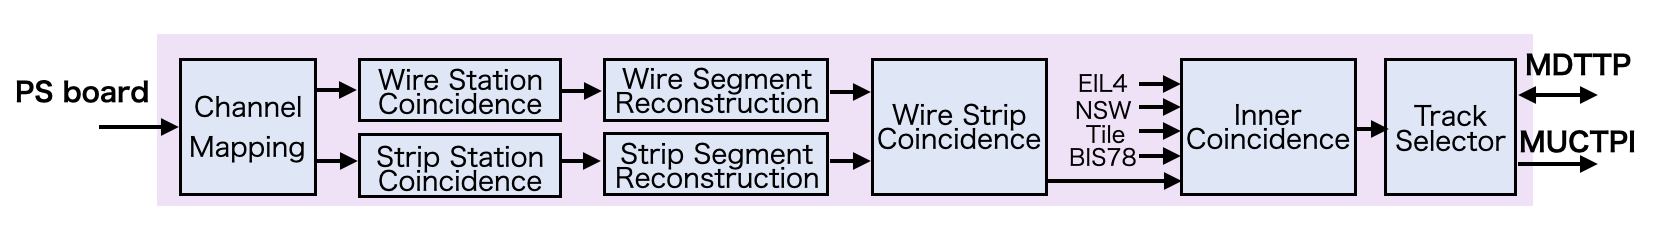
\includegraphics[width=16cm]{fig/SL/Trigger_over.png}
\caption[トリガー回路の全体像]{トリガー回路の全体像}
\label{Trigger_over}
\end{figure}

SL FPGAに実装されるトリガーロジックはChannel Mapping、Station Coincidence、Segment Reconstruction、Wire Strip Coincidence、Inner Coincidence、Track Selectorという6つのモジュールをパイプライン的に接続することで実現される。
PS board から受信するヒットビットマップはChannel Mapping でコインシデンスロジックの入力に適した形へと並び替えられる。入力されたヒットデータはStation CoincidenceおよびSegment reconstructionでワイヤー、ストリップそれぞれでコインシデンスがとられる。Segment Reconstruction ではTGCのヒットから再構成される飛跡と無限運動量飛跡のなす角d$\theta$、d$\phi$が計算される。Wire Strip coincidenceは、Wireで再構成されたd$\theta$とStripで再構成されたd$\phi$のコインシデンスを取ることで、横方向運動量閾値\pt を概算する。ここまでのコインシデンスロジックをまとめてTGC BW コインシデンスと飛ぶ。TGC BW コインシデンスで再構成されたミューオン飛跡候補はInner Coincidenceにて、磁場内部の検出機(NSW、BIS78、RPC、EIL4 TGC、Tile カロリメーター)とコインシデンスが取られ、フェイクトリガーの削減および\pt 精度の向上が実現される。Inner Coincidenceは最大112個の飛跡候補を出力する。最後にTrack selectorで、112個の飛跡候補から\pt の大きい順に最大6つの飛跡候補が選別される。そのうち3つはMDTTPに転送され、MDTTTPにてさらに高い精度でミューオンの運動量を計算された後、その結果を再度受け取る。SLはMDTTPから受信した飛跡候補3つと、MDTTPへ転送しなかった飛跡候補3つ合わせて6つをMUCTPIに転送する。以下にそれぞれのロジックの詳細と、HDLへの実装方法を説明する。

\subsection{Channel Mapping}
\subsubsection*{コンセプト}
Channel MappingではPS board から受信するTGC BW 全チャンネルのヒット情報 (128 bit x 62 link)を、飛跡再構成に先んじてトリガー入力に適したフォーマットへとマッピングする処理を行う。この工程ではただチャンネルを並び変えるだけでなく、TGC検出器のジオミトリに合わせて設計されたフロントエンドのチャンネル構造をトリガーロジックとして取り扱いやすいものへと変換する。TGC BW のエンドキャップ領域は$\eta$方向にM1は4つ、M2、M3は5つのチェンバーで構成されており、それぞれ不完領域がないようにオーバーラップを持って設置されている。このオーバーラップ領域では一つのミューオンのヒットを重複してカウントする可能性があるため、トリガーに入力する際にはWIred ORと呼ばれる統合処理を行う。また、ストリップのコインシデンスはチェンバーごとに行われるが、ミューオン飛跡が$\eta$方向に曲げられ、複数のチェンバーに跨ってヒットを残した場合には、コインシデンスをとることができない。これに対処するため、とあるM3チェンバーとのコインシデンスと担当するM1及びM2チェンバーでは図\ref{}のようにORを取った上で、コインシデンスが取られる。

\begin{figure} 
\centering
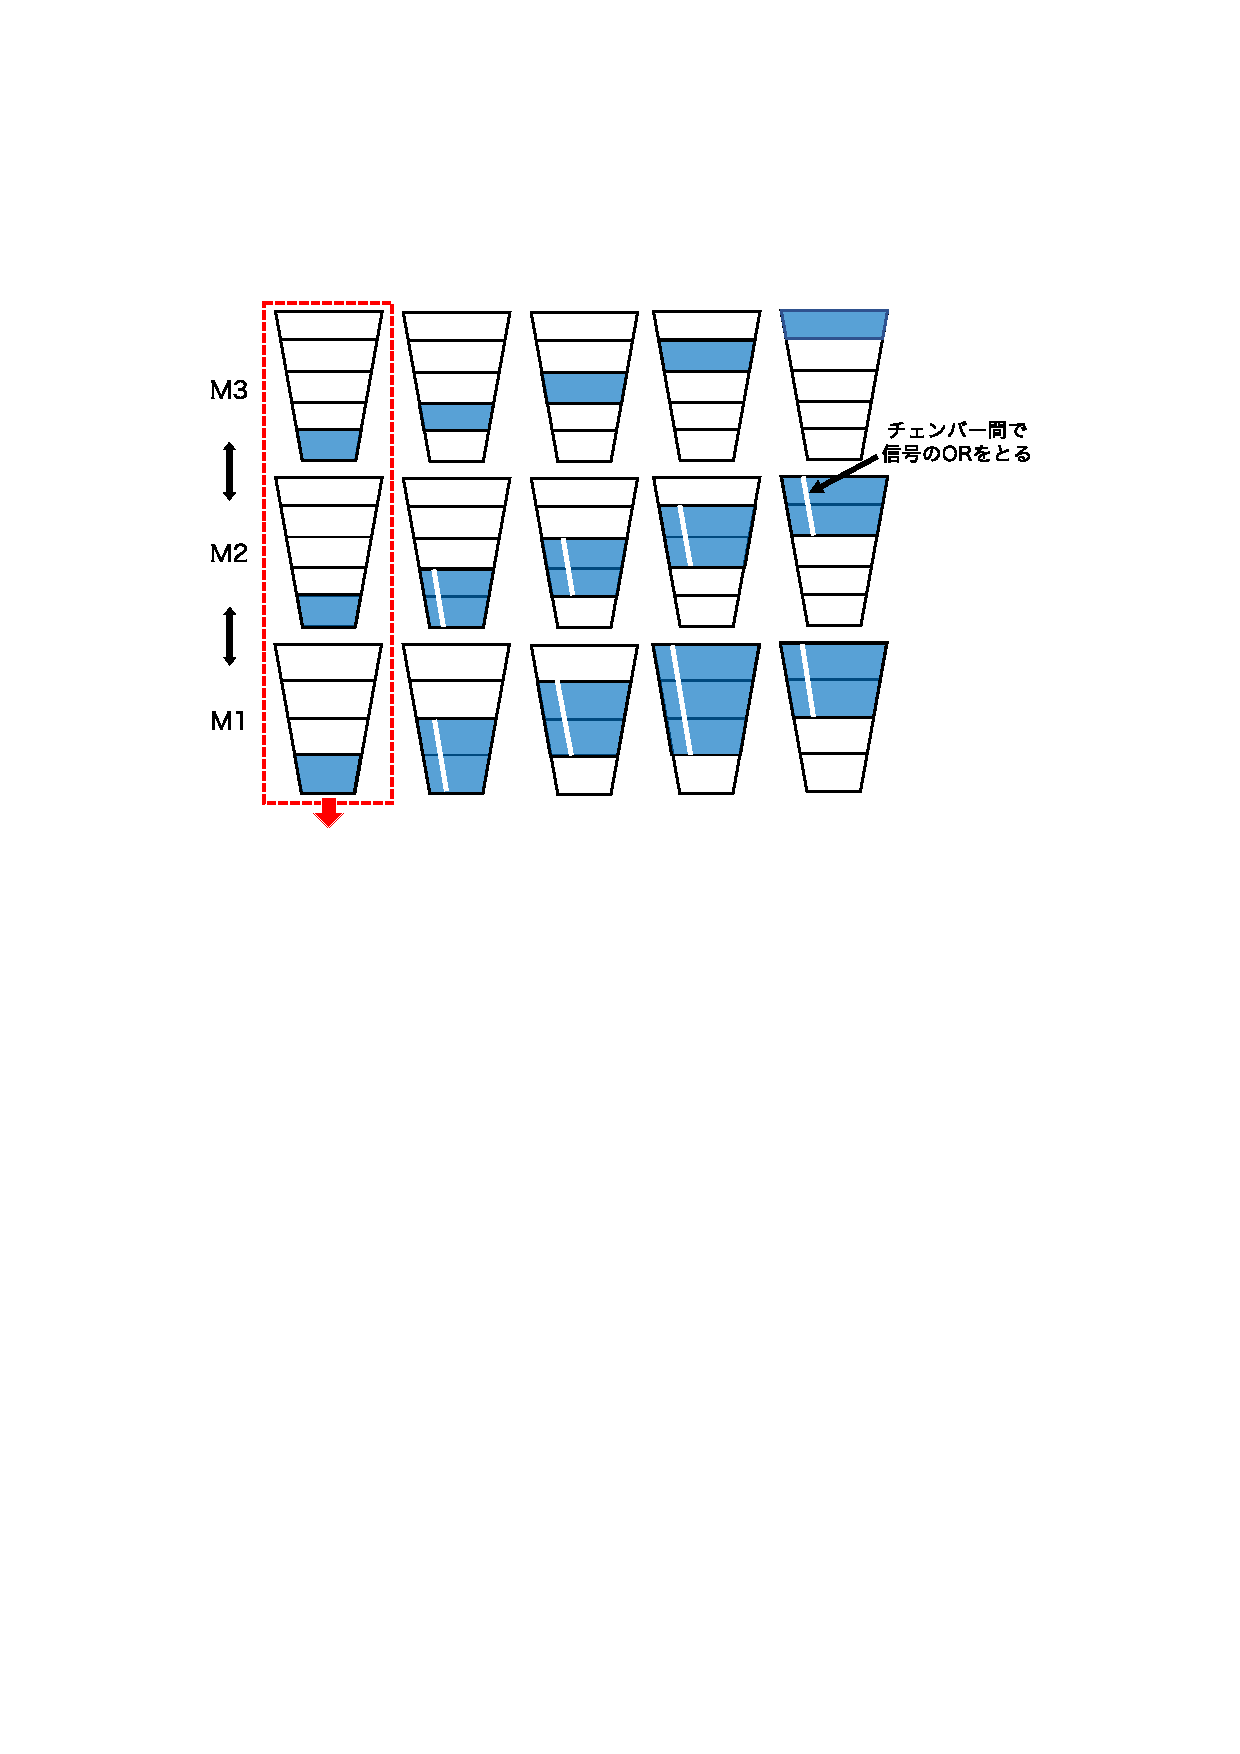
\includegraphics[width=16cm]{fig/SL/Channel_Mapping.pdf}
\caption[]{ストリップにおけるチェンバー間のORの取り方。M3チェンバーとのコインシデンスと担当するM1及びM2チェンバーではORをとった情報を後段に流す。\cite{mt_kawamoto}}
\label{fig_CTA}
\end{figure}

\subsubsection*{HDL実装}
Channel MappingモジュールはHDLでは単純な配線とOR回路で実装されている。

\subsection{Station Coincidence}
\subsubsection*{コンセプト}
図\ref{}にStation Coincidenceの概要を示す。TGC検出器はスタッガリング構造を取っており、ステーション内のワイヤーは互いに$\eta$方向にずらして、ストリップは互いに$\phi$方向にずらして設置されている。M1、M2、M3の各チャンネルが重複してカバーする$\eta$領域、$\phi$領域を代表点として定義する。Station CoincidenceはM1 3層、M2 2層、M3 2層のヒットチャンネルを入力として、コインシデンスが取れた代表点を出力する。これによりデータ量を落としながら、より位置分解能を上げてミューオンの位置情報を決めることができる。

\begin{figure} 
\centering
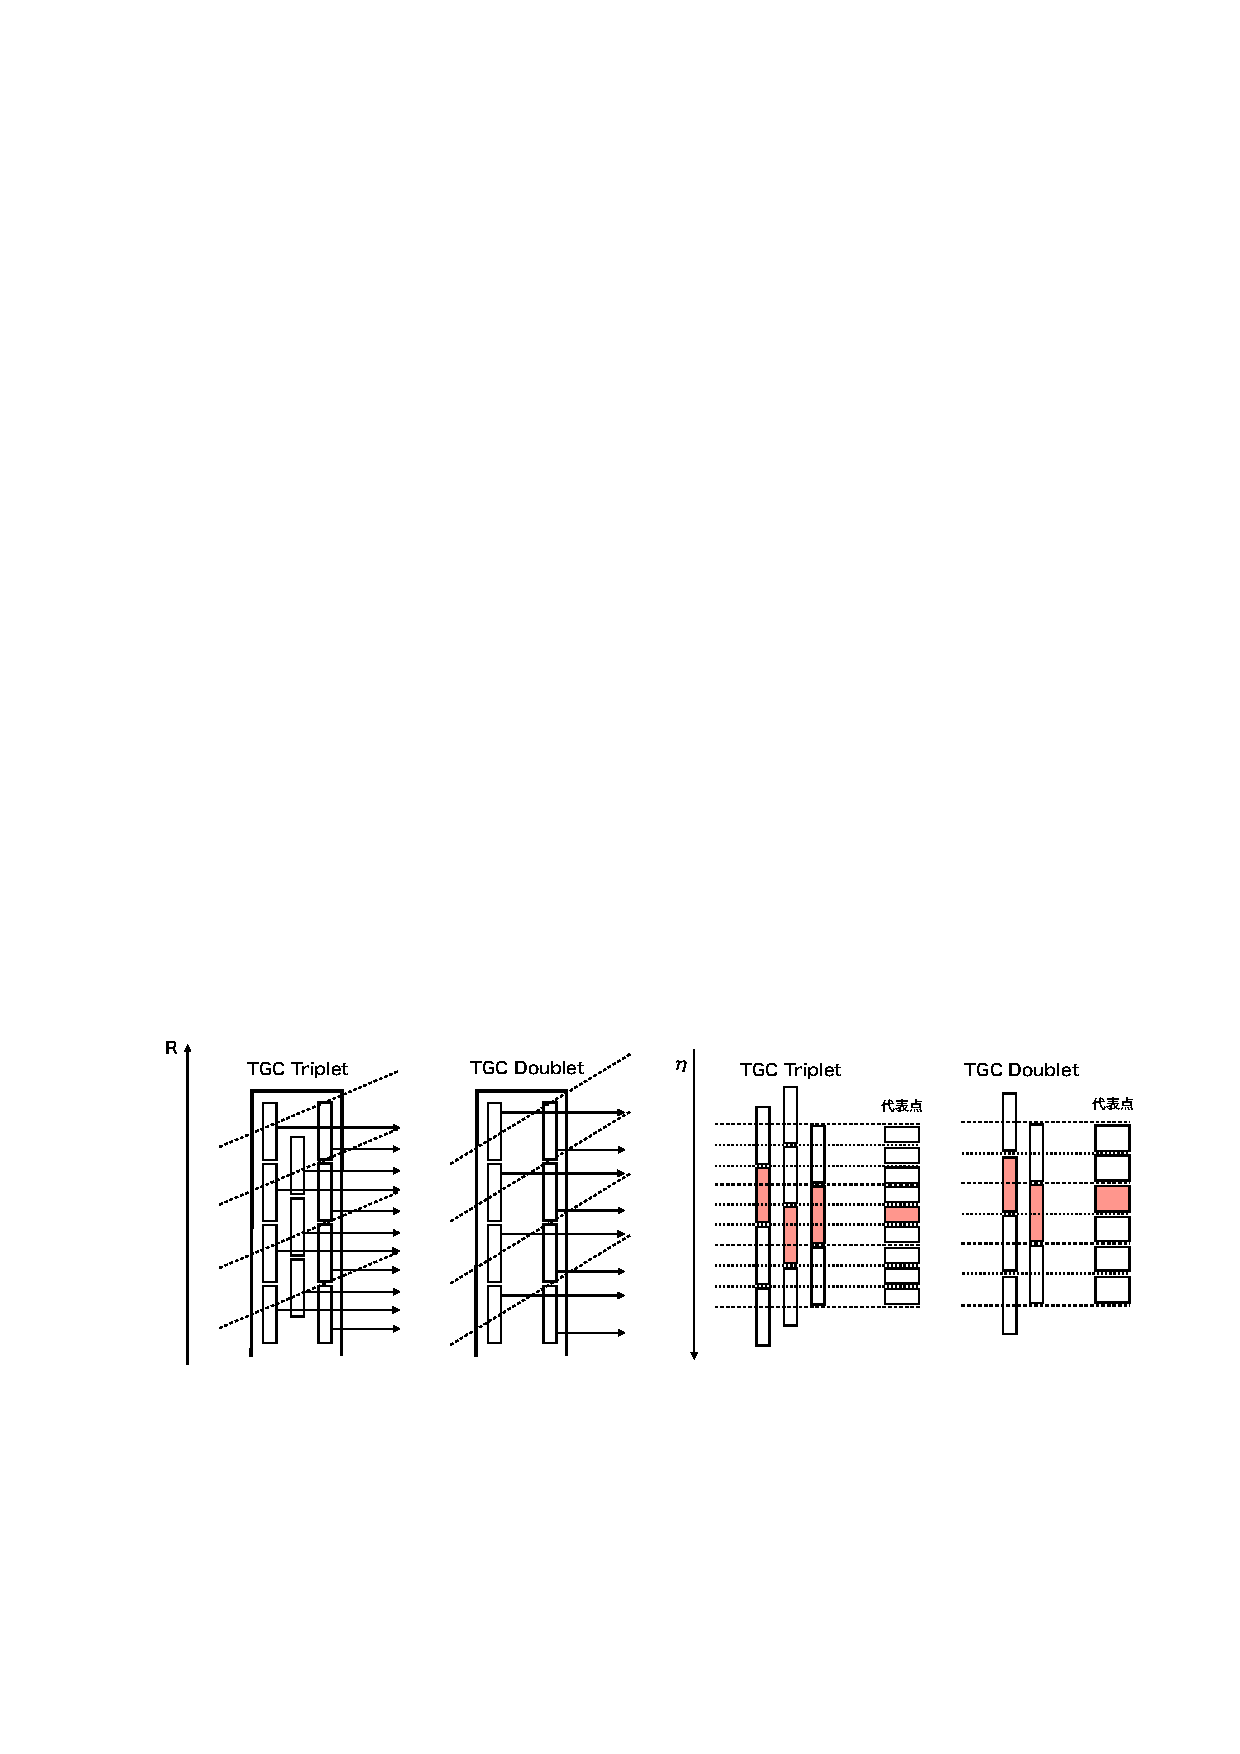
\includegraphics[width=16cm]{fig/SL/Concept_station.pdf}
\caption[Station コインシデンスの概要]{Station コインシデンスの概要\cite{mt_mino}。スタッガリング構造をとっている。}
\label{Concept_station}
\end{figure}

\subsubsection*{Wire Station CoincidenceのHDL実装}
このモジュールの駆動クロックは、LHCバンチ交差クロックに同期した40 MHzクロックでレイテンシーは1クロックチック ( 25 ns )である。
Wire Station Coincidenceおよび\ref{subsec:segment_reco}節で説明するWire Segment ReconstructionはUnit、Subunitと呼ばれる単位領域でトリガーセクターを分割して、Subunitごとに並列にコインシデンス処理を行う。UnitやSubunitは先行研究にて、とあるM3チャンネルにヒットを残した\pt 5 GeVのミューオンを再構成するのに必要な、M1、M2チャンネルを網羅するよう定義された。

ワイヤーロジックではエンドキャップ領域を37分割、フォワード領域を16分割したものをUnitと定義する。図\ref{StationCoin_unit}にユニットの構造を示す。1つのユニットはM1ステーションの96 代表点、M2ステーションの32代表点、M3ステーションの16代表点をカバーする。また、1つのユニットを4等分するようにしてSubunitが定義されている。

\begin{figure} 
    \centering
    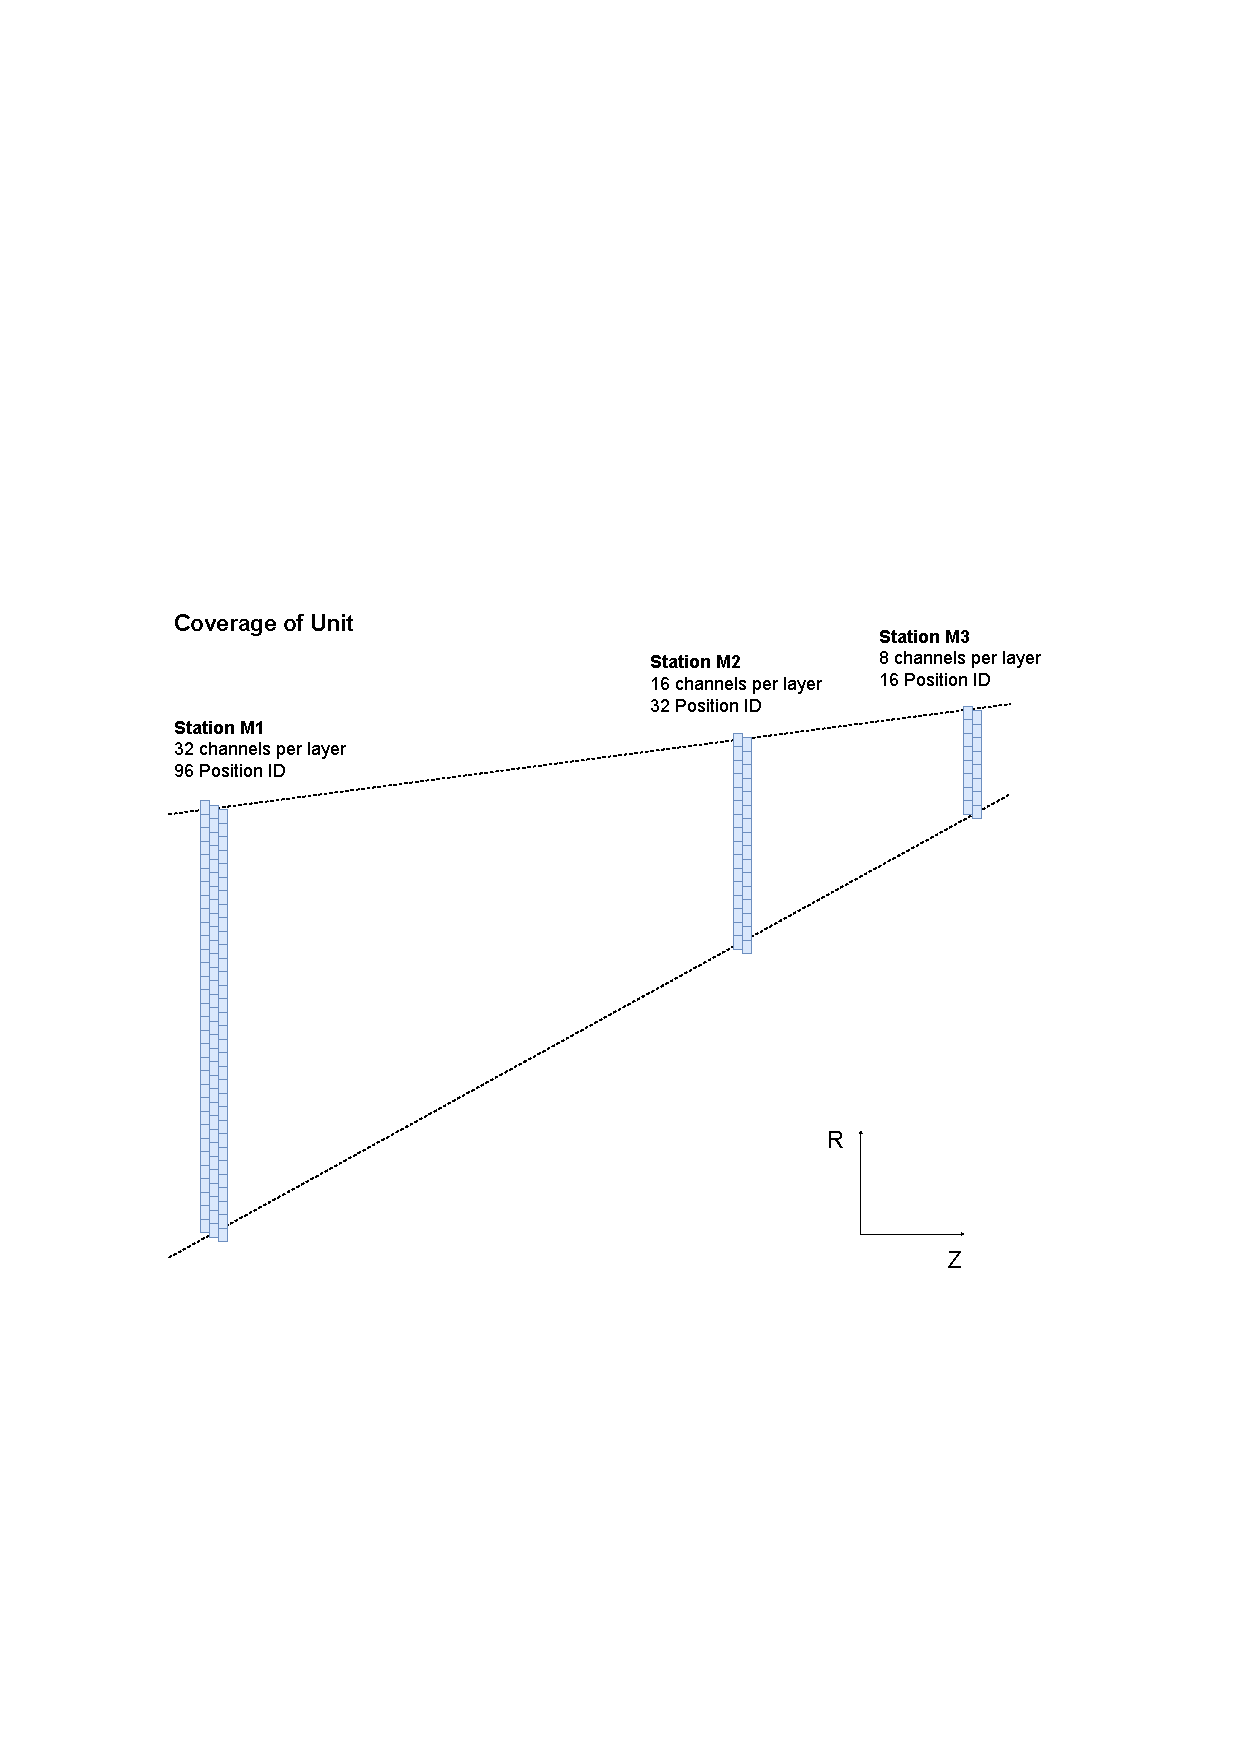
\includegraphics[width=16cm]{fig/SL/StationCoin_unit.pdf}
    \caption[Wire Station Coincidence および Wire Segment Reconstruction におけるユニット]{Wire Station Coincidence および Wire Segment Reconstruction におけるユニット}
    \label{StationCoin_unit}
\end{figure}

M1ステーションにおけるコインシデンスロジックの概要を図\ref{StationCoin_wire}に示す。ステーションコインシデンスはHDLではandとorの組み合わせ回路として実装される。3層中3層にヒットがあった場合に代表点を出力する3/3コインシデンス、2層にヒットがあった場合の2/3コインシデンス、1層にヒットがある場合の1/3コインシデンスが独立に用意されており、それぞれが並列に動作する。

\begin{figure} 
    \centering
    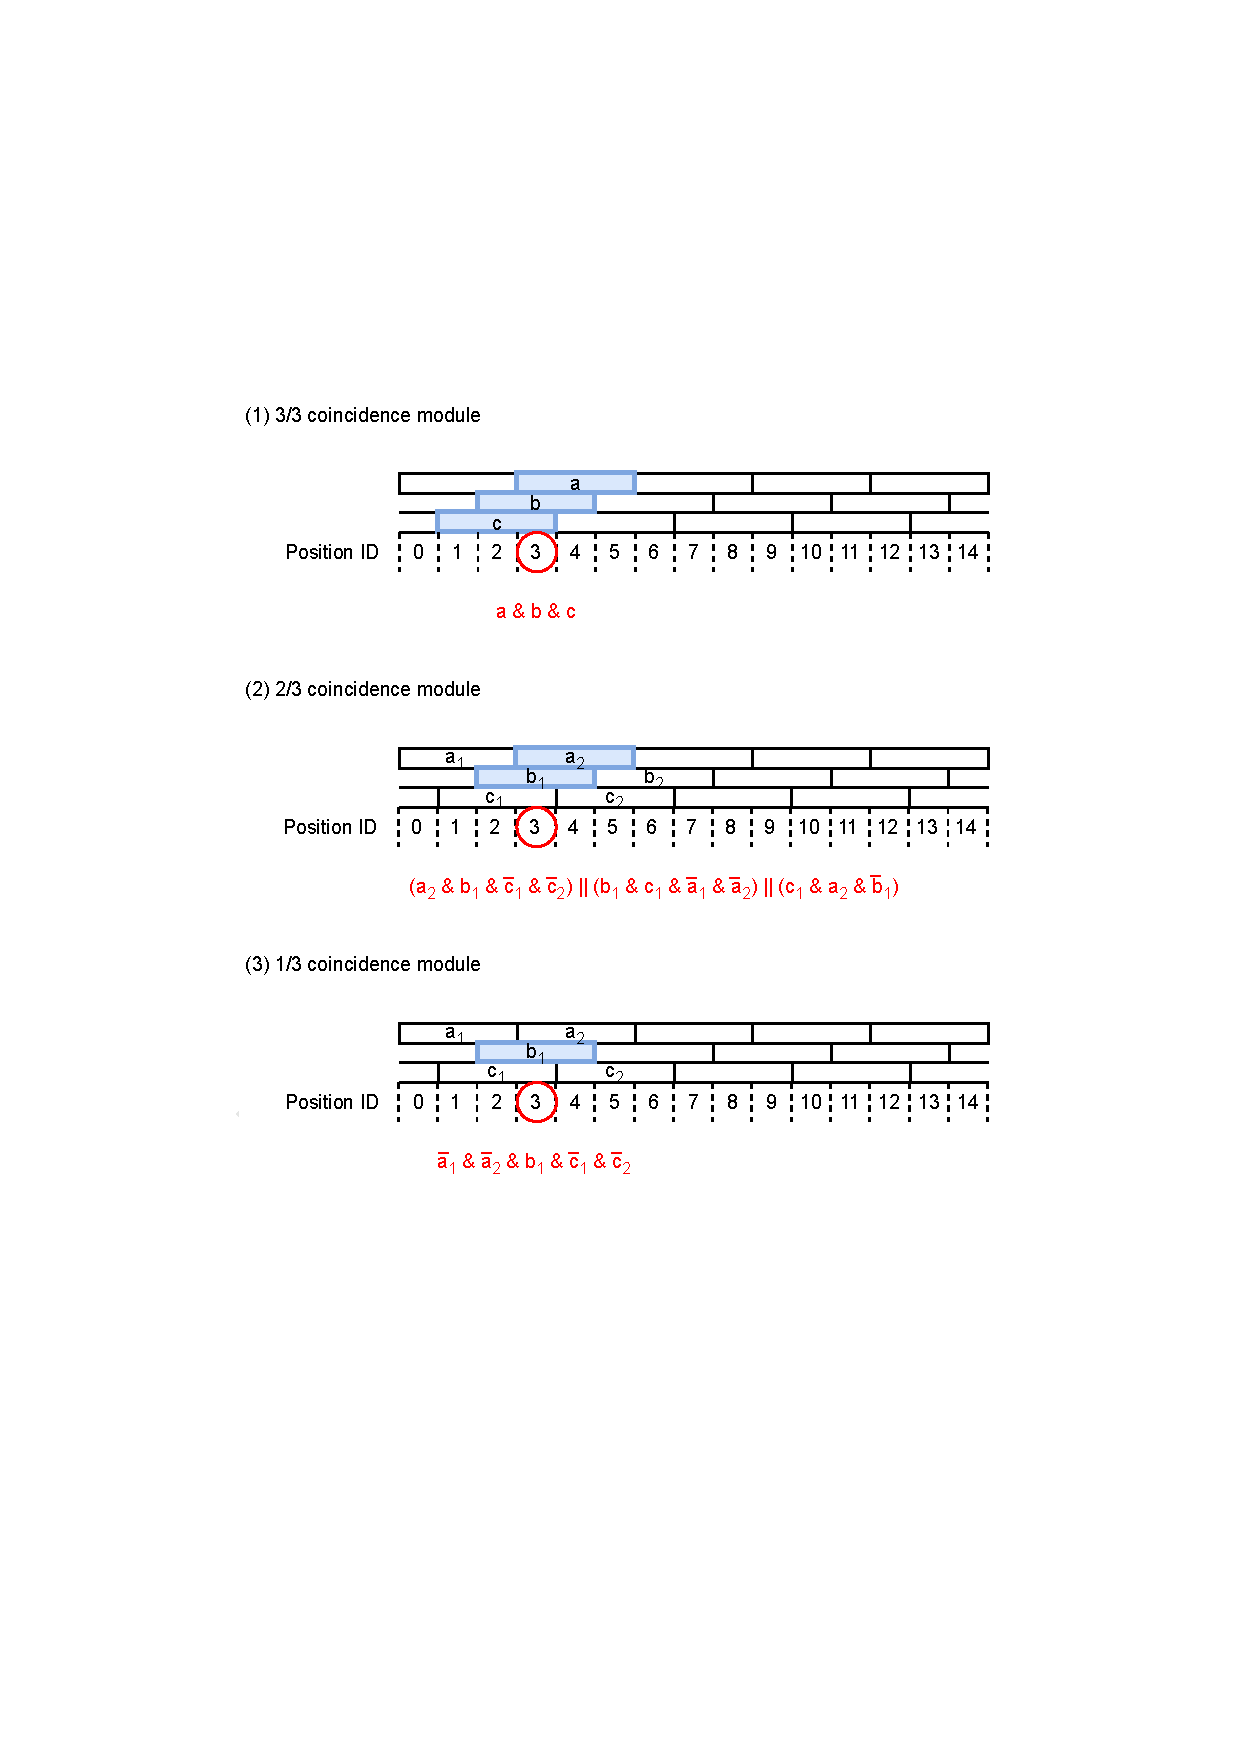
\includegraphics[width=16cm]{fig/SL/StationCoin_wire.pdf}
    \caption[M1 tripletにおけるコインシデンスロジック]{M1 tripletにおけるコインシデンスロジック}
    \label{StationCoin_wire}
\end{figure}

M2、M3ステーションは2層で構成されているため、2/2コインシデンスと1/2コインシデンスが用意されており、それぞれのロジックは図\ref{StationCoin_doublet}のように実装される。
    
\begin{figure} 
\centering
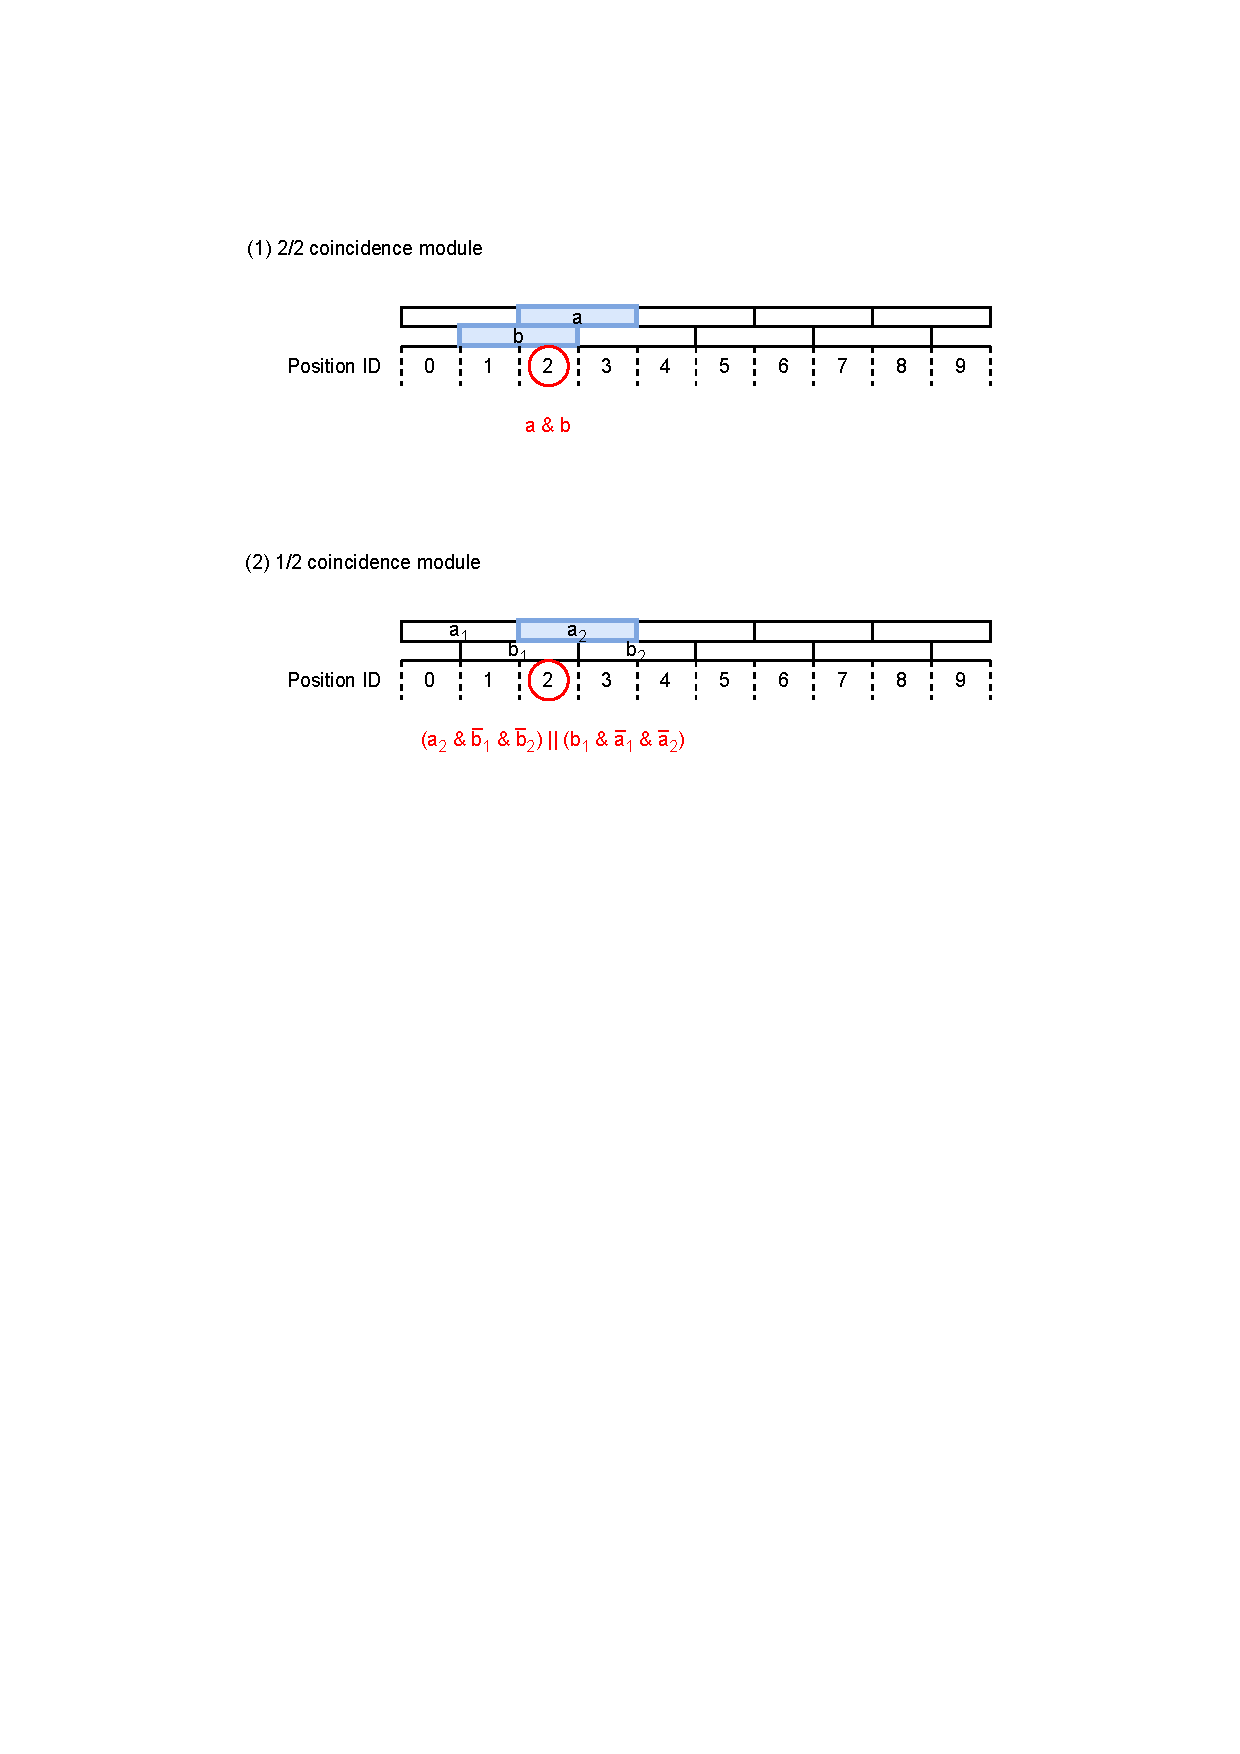
\includegraphics[width=16cm]{fig/SL/StationCoin_doublet.pdf}
\caption[M2・M3 ステーションにおけるコインシデンスロジック]{M2・M3 ステーションにおけるコインシデンスロジック}
\label{StationCoin_doublet}
\end{figure}

各コインシデンスロジックで、複数の代表点が出力された場合には各サブユニットごとに後段に送る代表点を選別する。M1、M2ステーションでは検出器がユニットの中心により近いものが2つ、M3ステーションでは$\eta$がより小さいものが1つ選ばれる。これらのロジックはより大きな\pt のミューオンを通すことを目的に、ソフトウェアでのシミュレーションなどを経て最適化されたものである。
% ステーションコインシデンスの最終的な出力は図\ref{}のテーブルのようにまとめらる。

\subsubsection*{Strip Station CoincidenceのHDL実装}
このモジュールの駆動クロックは、LHCバンチ交差クロックに同期した40 MHzクロックでレイテンシーは1クロックチック ( 25 ns )である。Strip Station Coincidenceおよび\ref{subsec:segment_reco}節で説明するStrip Segment ReconstructionもUnit、Subunit呼ばれる単位領域でトリガーセクターを分割して、Subunitごとに並列にコインシデンスロジックを走らせる。Strip では 1つのチェンバーを4分割するようユニットが定義される。エンドキャップ領域は5枚のチェンバーで構成されるため20 Unit、フォワード領域は1枚のチェンバーで構成されるため5 unit 存在する。図\ref{StationCoin_unit_strip}にユニットの構造を示す。1つのユニットはM1ステーションの40 代表点、M2ステーションの24代表点、M3ステーションの16代表点をカバーする。また、1つのユニットを2等分するようにしてSubunitが定義されている。

\begin{figure} 
    \centering
    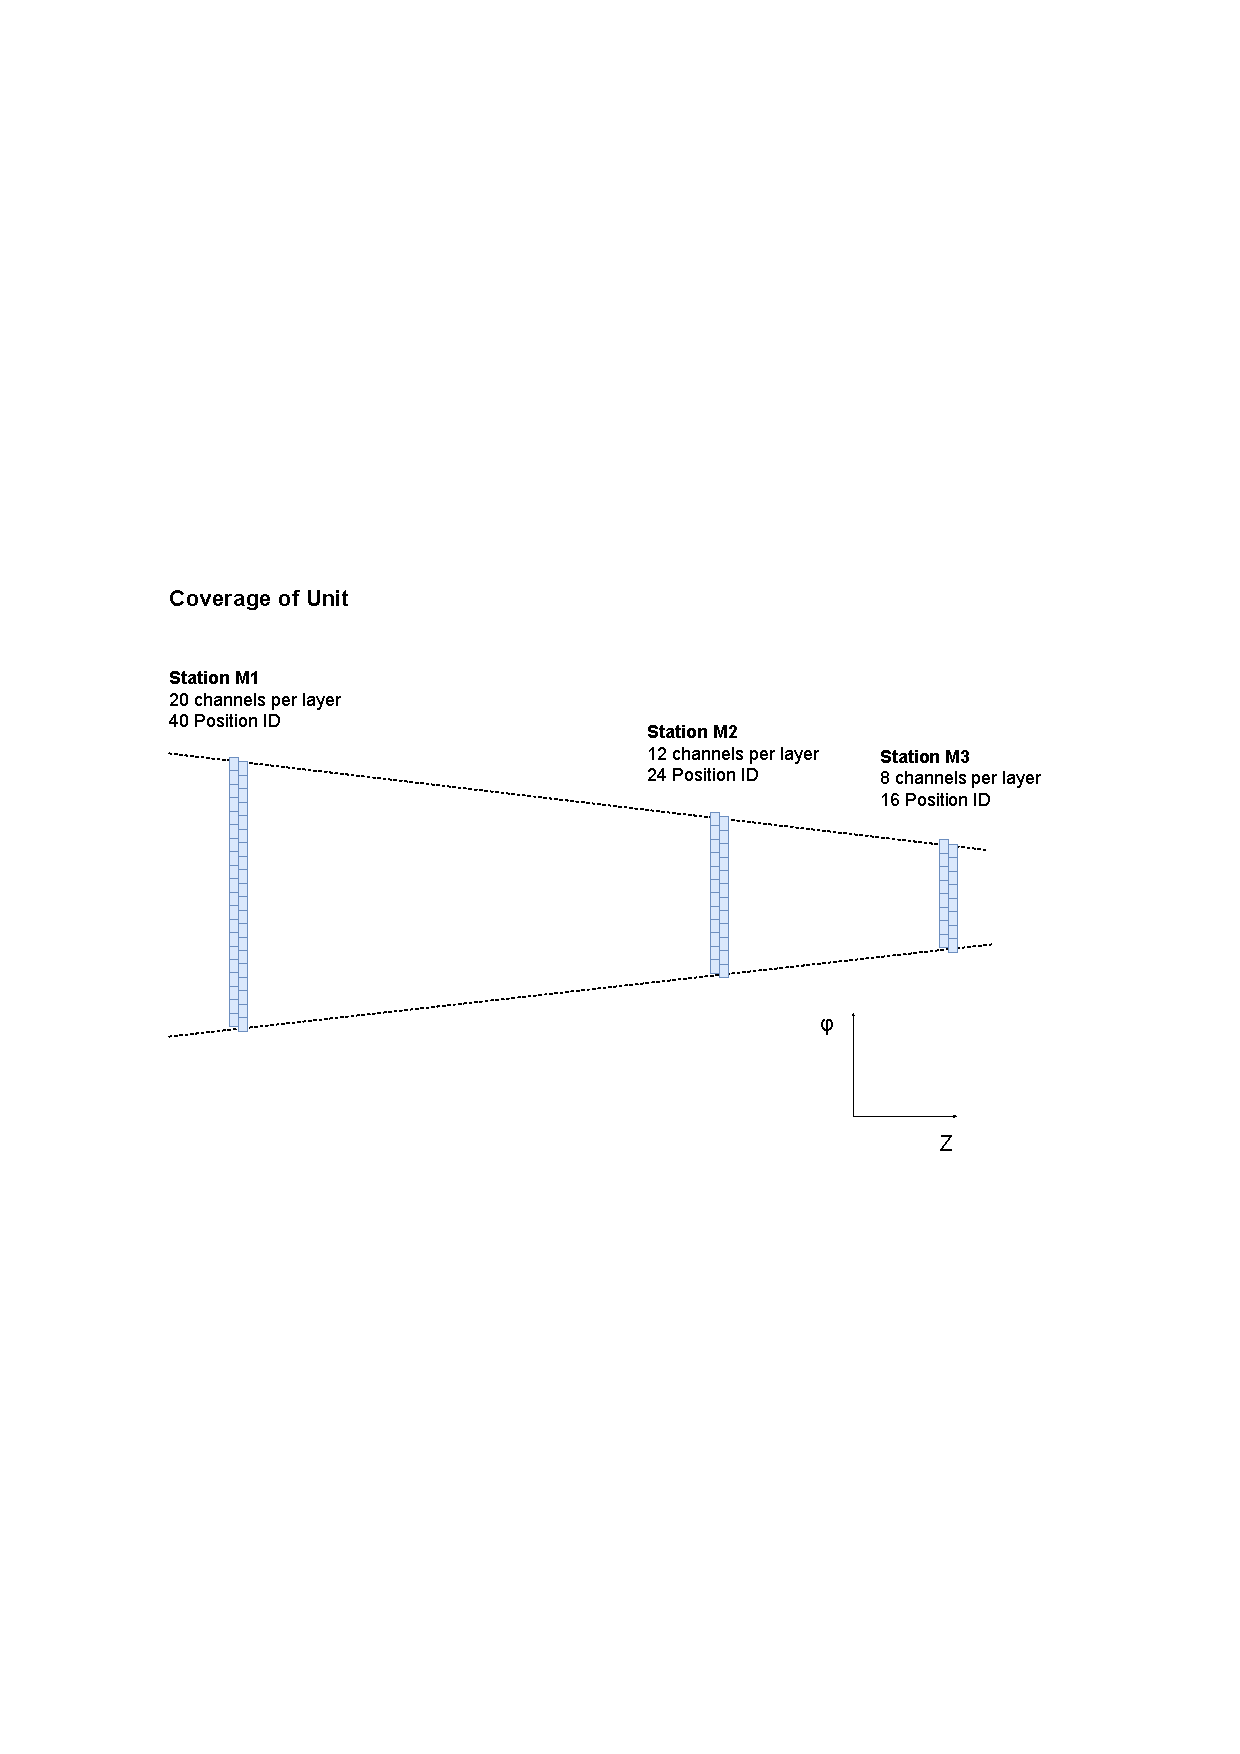
\includegraphics[width=16cm]{fig/SL/StationCoin_unit_strip.pdf}
    \caption[Strip Station Coincidence および Strip Segment Reconstruction におけるユニット]{Strip Station Coincidence および Strip Segment Reconstruction におけるユニット}
    \label{StationCoin_unit_strip}
\end{figure}

コインシデンスのロジックは基本的にワイヤーと同じで、M1、M2、M3ともに2層構造になっているためそれぞれ2/2、1/2ロジックが並列に走っている。
% 最終的な出力は図\ref{}のようにまとめられ、後段に送られる。


\subsection{Segment Reconstruction}
\label{subsec:segment_reco}
\subsubsection*{コンセプト}
Segment Reconstructionではステーションコインシデンスで取り出された、各ステーションの代表点の組み合わせから、無限運動量飛跡と実際の飛跡のなす角度 ($\Delta\theta$、$\Delta\phi$)を算出する。Segment Reconstructionの概念図を図\ref{Concept_segment}に示す。角度情報の概算には、パターンマッチングと呼ばれる手法を用いる。この手法ではあらかじめ、代表点の組み合わせとそこから計算される角度情報の対応関係をまとめたテーブル (パターンリスト、LUTともよぶ) を用意することで、複雑な計算をせずとも高速で角度情報を再構成する。

\begin{figure} 
\centering
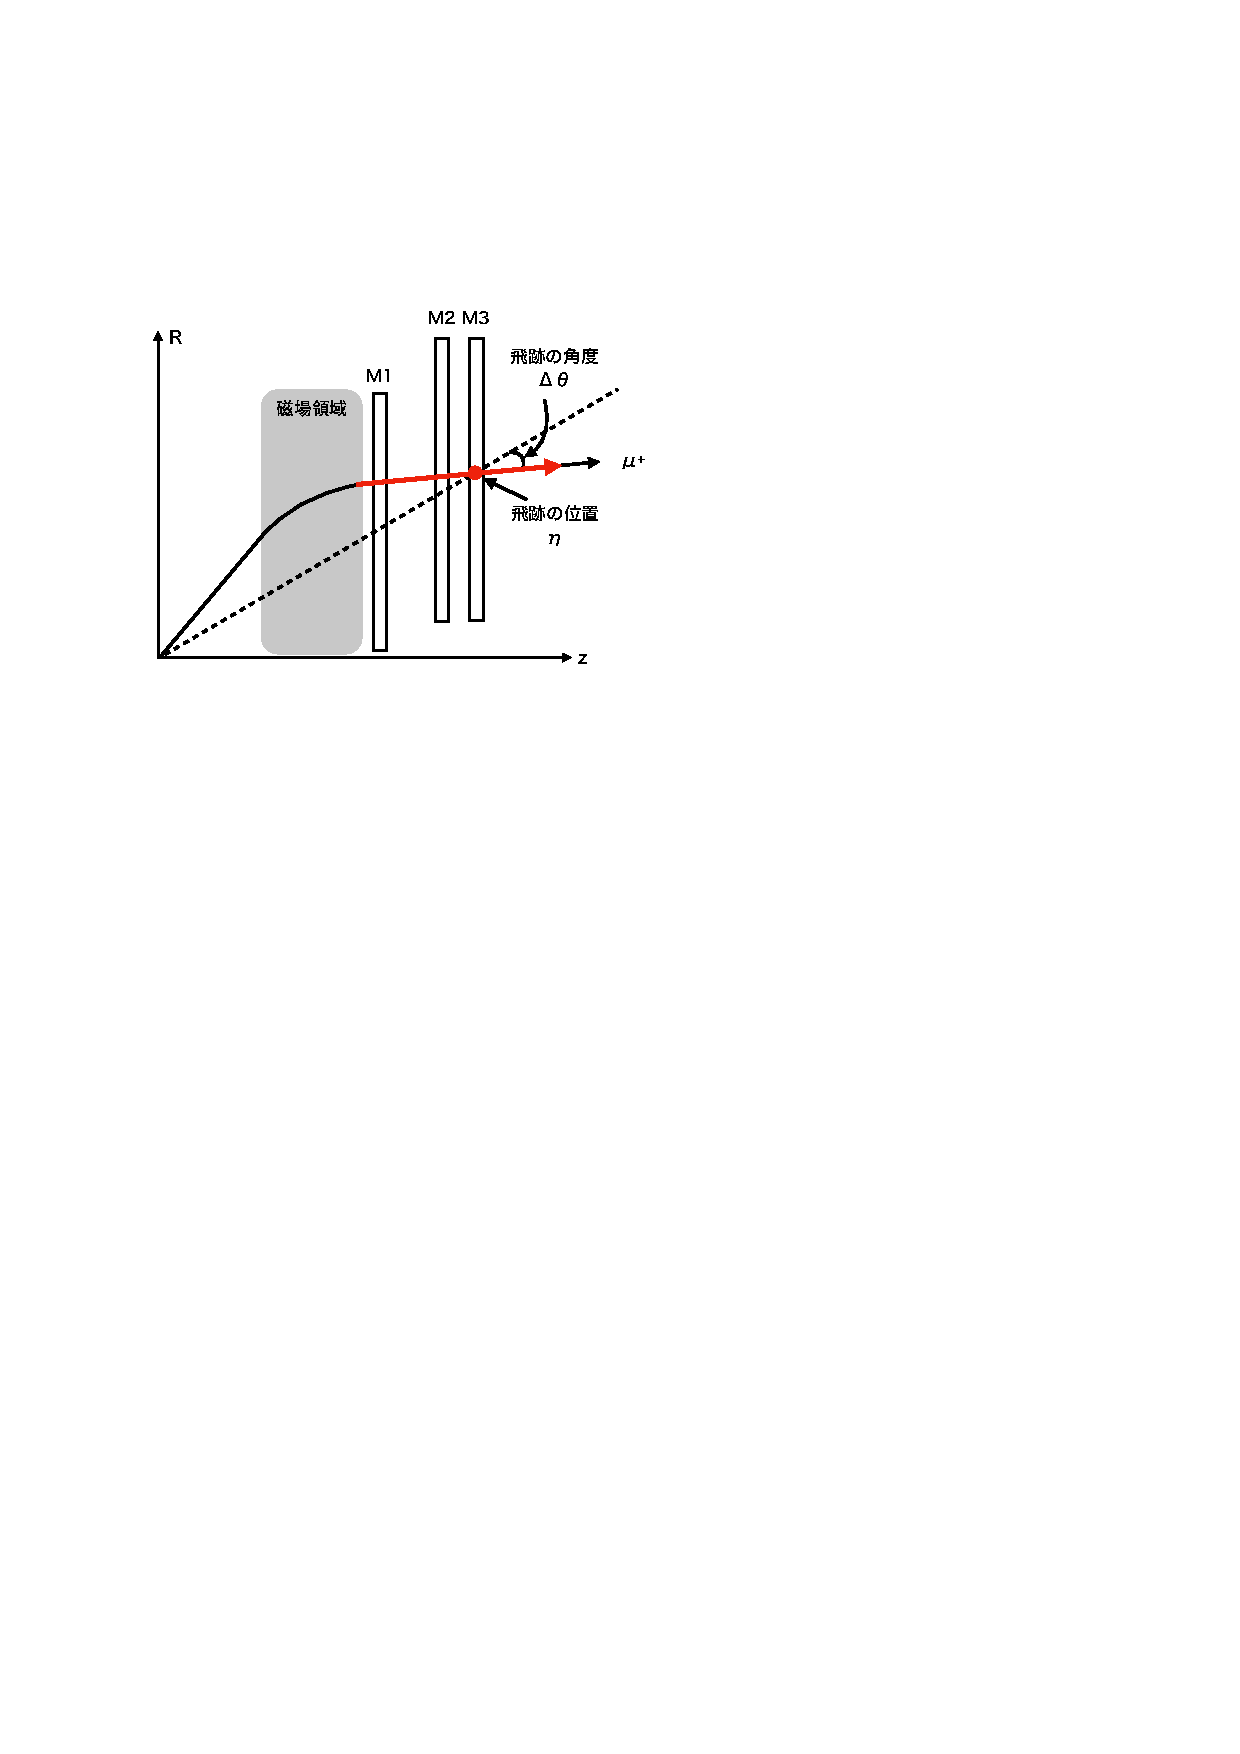
\includegraphics[width=16cm]{fig/SL/Concept_segment.pdf}
\caption[Segment Reconstructionのコンセプト]{$\eta$方向 (左) および$\phi$方向 (右) のパターンマッチングの概念図\cite{mt_mino}。黒い線が実際のミューオンの飛跡を表し、赤い線がTGCのヒットから再構成される飛跡を表す。黒い点線はM3ステーションの代表点と衝突点を結んだ、無限運動量飛跡を表し、再構成した飛跡と無限運動量飛跡との角度をパターンとして保存する。}
\label{Concept_segment}
\end{figure}

\subsubsection*{Wire Segment ReconstructionのHDL実装}
このモジュールの駆動クロックは、LHC クロックに同期した周波数 160 MHz のクロックであり、レイテンシは 12 クロックチック分 (75 ns) である。
Wire Segment Reconstructionではサブユニットごとに1つLUTが用意され、サブユニット内のM1、M2、M3代表点を組み合わせることでパターンマッチングを行う。最終的にはそれぞれのサブユニットから最大1つの飛跡情報を出力するため、SL全体では最大360の角度情報が出力される。Wire Segment Reconstructionの各サブユニット内でのロジックの概要を図\ref{SegReco_wire}に示す。各サブユニットはAddress Specifier・Segment Extractor・Segment Selector で構成される。以下でそれぞれのモジュールについて述べる。

\begin{figure} 
\centering
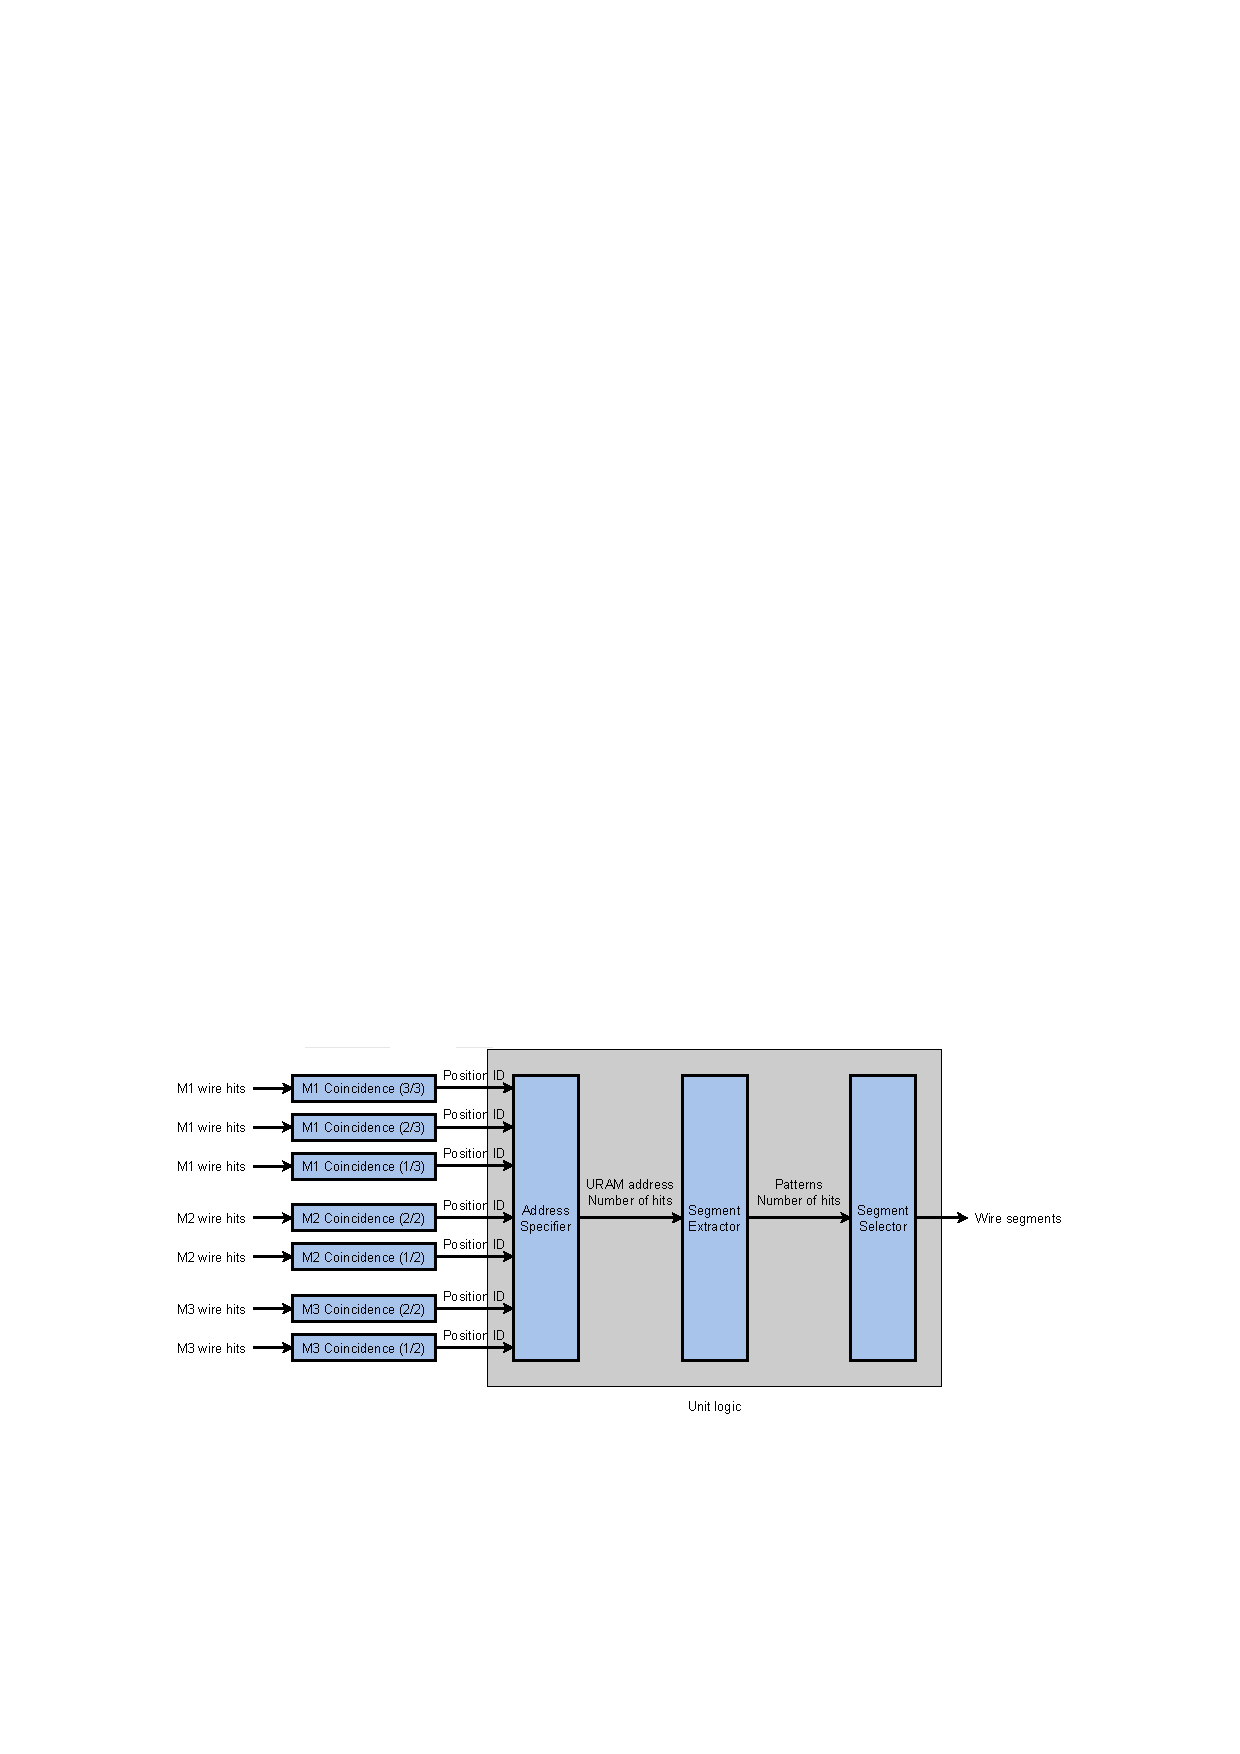
\includegraphics[width=16cm]{fig/SL/SegReco_wire.pdf}
\caption[Wire Segment Reconstructionのブロックダイアグラム]{Wire Segment Reconstructionのブロックダイアグラム\cite{SLPDR}}
\label{SegReco_wire}
\end{figure}

\subsubsection*{Address Specifier}
Wire Station Coincidenceで得られた各ステーションの代表点を組み合わせて、LUT にアクセスするためのアドレスを作成する。ステーションコインシデンスからは最大M1 個 6個、M2 4個、M3 2個の代表点が送られるため、最大 6 x 4 x 2 = 48 パターンの組み合わせが取られるが、この中から8つのパターンを選抜してSegment Extractorへ送る。パターンを選択する際にはマッチレイヤーが多いもの優先する。具体的に優先順位を定めたテーブルを表\ref{tab:StationCoin_wire}に示す。より上位にリストされているコインシデンスパターンが優先して送られる。また同じコインシデンスパターンが複数存在する場合には、$\eta$がより小さいものが選ばれる。この選び方もソフトウェアシミュレーションによる先行研究に基づいており、こうすることでより高い角度分解能で飛跡を再構成できることがわかっている。なお、同表中のFractionの値はミューオンがガスレイヤーを通過した時にヒットを残す確率を94 \%と仮定して算出したものである。

\begin{table}[h]
    \centering
    \caption{Wire Station Coincidenceにおけるコインシデンスパターン}
    \label{tab:StationCoin_wire}
    \begin{tabular}{|cc|c|}
    \hline
    \multicolumn{1}{|c|}{\multirow{2}{*}{Coincidence Pattern}} & Hit Pattern & \multirow{2}{*}{Faraction} \\ \cline{2-2}
    \multicolumn{1}{|c|}{}                                     & M1 M2 M3    &                            \\ \hline\hline
    \multicolumn{1}{|c|}{7/7}                                  & 3/3 2/2 2/2 & 0.649                      \\ \hline
    \multicolumn{1}{|c|}{6/7A}                                 & 2/3 2/2 2/2 & 0.124                      \\ \hline
    \multicolumn{1}{|c|}{6/7B}                                 & 3/3 1/2 2/2 & 0.083                      \\ \hline
    \multicolumn{1}{|c|}{6/7C}                        & 3/3 2/2 1/2 & 0.083                      \\ \hline
    \multicolumn{1}{|c|}{5/7A}                                 & 2/3 1/2 2/2 & 0.016                      \\ \hline
    \multicolumn{1}{|c|}{5/7B}                                 & 1/3 2/2 1/2 & 0.016                      \\ \hline
    \multicolumn{1}{|c|}{5/7C}                                 & 3/3 1/2 1/2 & 0.011                      \\ \hline
    \multicolumn{1}{|c|}{5/7D}                                 & 1/3 2/2 2/2 & 0.008                      \\ \hline\hline
    \multicolumn{2}{|c|}{Total}                                              & 0.988                      \\ \hline
    \end{tabular}
\end{table}

\subsubsection*{Segment Extractor}
Wire Segment Reconstructionで利用されるLUTはFPGAのURAM上に格納される。Segment ExtractorではAddress Specifierで作られたアドレスをもとに、URAMにアクセスし、対応するデータ (Wire Segment) を出力する。Wire Segmentのデータフォーマットを表\ref{tab:WireSegment}に示す。URAMはdual portで設計されており、1つのサブユニットが2ポート利用する。そのため1つのサブユニットは40 MHz クロック 1チックの間で 8つのデータを処理する。

\begin{table}[h]
    \centering
    \caption{Wire Segmentのフォーマット}
    \label{tab:WireSegment}
    \begin{tabular}{|c|c|}
    \hline
    \# of bits & Name                                                                       \\ \hline\hline
    1          & Flag of successful reconstruction                                          \\ \hline
    2          & Number of the stations with hits used for coincidence                      \\ \hline
    8          & Angle difference $\Delta\theta$ between the segment and the vector from IP \\ \hline
    12         & Global $\eta$ position of the segment                                      \\ \hline
    \end{tabular}
\end{table}

\subsubsection*{Segment Selector}
Segment Extractorから送られる最大8つのWire Segment から マッチレイヤーの多さを基準に最大1つ選択して、Wire Strip Coincidence へと送信する。マッチレイヤーも同じものが複数ある場合には$\Delta\theta$がより小さいものを選ぶ。

\subsection*{Strip Segment Reconstruction}
このモジュールの駆動クロックは、LHC クロックに同期した周波数 240 MHz のクロックであり、レイテンシーは 21 クロックチック分 (87.5 ns) である。
Strip Segment Reconstructionではサブユニットごとに1つLUTが用意され、サブユニット内の代表点を組み合わせることでパターンマッチングを行う。最終的にはユニット内の2つのサブユニット合わせて、1つの角度情報が出力される。SL全体では最大45の飛跡情報が出力される。Strip Segment Reconstructionの各サブユニット内でのロジックの概要を図\ref{SegReco_strip}に示す。各サブユニットはAddress Specifier・Segment Extractor・Segment Selector で構成される。以下でそれぞれのモジュールについて述べる。

\begin{figure} 
\centering
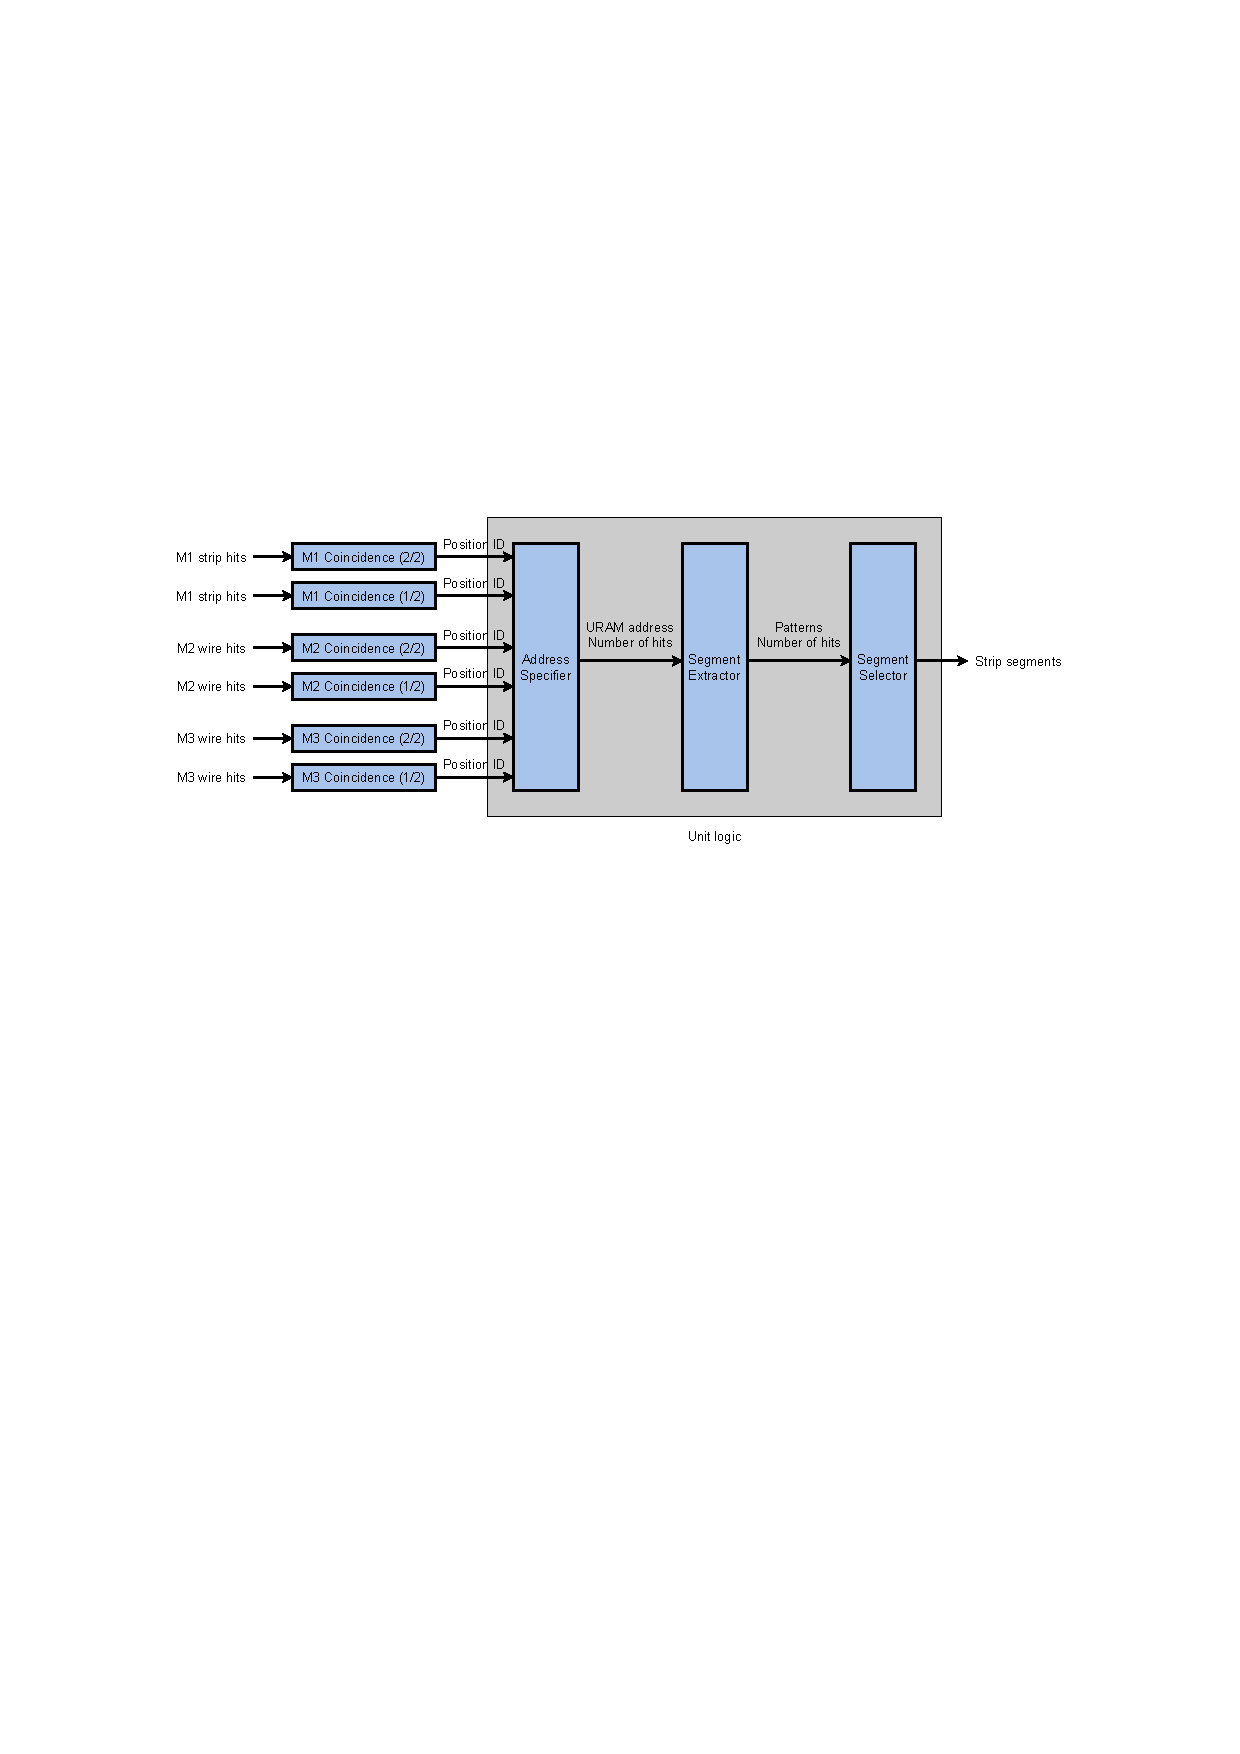
\includegraphics[width=16cm]{fig/SL/SegReco_strip.pdf}
\caption[Strip Segment Reconstruction のブロックダイアグラム]{Strip Segment Reconstruction のブロックダイアグラム}
\label{SegReco_strip}
\end{figure}

\subsubsection*{Address Specifier}
Strip Station Coincidenceで得られた各ステーションの代表点を組み合わせて、LUT にアクセスするためのアドレスを作成する。ステーションコインシデンスからは最大M1 個 4個、M2 4個、M3 2個の代表点が送られるため  4 x 4 x 2 = 32 パターンの組み合わせが取られうるが、この中から6つのパターンを選抜してSegment Extractorへ送る。パターンを選択する際にはワイヤーのロジックと同様にマッチレイヤーが多いもの優先する。具体的に優先順位を定めたテーブルを表\ref{tab:SegmentReco_strip}に示す。

\begin{table}[]
    \centering
    \caption{Strip Segment Reconstructionにおけるwire segmentのデータフォーマット}
    \label{tab:SegmentReco_strip}
    \begin{tabular}{|cc|}
    \hline
    \multicolumn{1}{|c|}{\multirow{2}{*}{Coincidence Pattern}} & Hit Pattern \\ \cline{2-2} 
    \multicolumn{1}{|c|}{}                                     & M1 M2 M3    \\ \hline\hline
    \multicolumn{1}{|c|}{6/6}                                  & 2/2 2/2 2/2 \\ \hline
    \multicolumn{1}{|c|}{5/6A}                                 & 2/2 1/2 2/2 \\ \hline
    \multicolumn{1}{|c|}{5/6B}                                 & 1/2 2/2 2/2 \\ \hline
    \multicolumn{1}{|c|}{5/6C}                                 & 2/2 2/2 1/2 \\ \hline
    \multicolumn{1}{|c|}{4/6A}                                 & 1/2 1/2 2/2 \\ \hline
    \multicolumn{1}{|c|}{4/6B}                                 & 2/2 1/2 1/2 \\ \hline
    \multicolumn{1}{|c|}{4/6C}                                 & 1/2 2/2 1/2 \\ \hline\hline
    \multicolumn{2}{|c|}{Total}                                              \\ \hline
    \end{tabular}
\end{table}

\subsubsection*{Segment Extractor}
Strip Segment Reconstructionで利用されるLUTはFPGAのURAM上に格納される。Segment ExtractorではAddress Specifierで作られたアドレスをもとに、URAMにアクセスし、対応するデータ (Strip Segment) を出力する。Strip Segmentのデータフォーマットを表\ref{tab:StripSegment}に示す。URAMはdual portで設計されており、2つのサブユニットが1ポートずつ利用する。そのため1つのサブユニットは、40 MHzクロック 1チックの間に6つのデータを処理する。

\begin{table}[]
    \centering
    \caption{Strip Segmentのフォーマット}
    \label{tab:StripSegment}
    \begin{tabular}{|c|c|}
    \hline
    \# of bits & Name                                                                     \\ \hline\hline
    2          & Number of the stations with hits used for coincidence                    \\ \hline
    6          & Local $\phi$ position in the chamber                                     \\ \hline
    9          & Angle difference $\Delta\phi$ between the segment and the vector from IP \\ \hline
    \end{tabular}
\end{table}

\subsubsection*{Segment Selector}
Segment Extractorから送られる最大6つのStrip Segment から マッチレイヤーの多さを基準にユニットごとに最大1 Segment 選択して、Wire Strip Coincidence へと送信する。マッチレイヤーも同じものが複数ある場合には$\Delta\phi$がより小さいものを選ぶ。

\subsection{Wire-Strip Coincidence}
\subsubsection*{コンセプト}
Wire Strip CoincidenceではWire Segment Reconstructionで算出した$\Delta\eta$とStrip Segment Reconstructionで算出した$\Delta\phi$を組み合わせることで、横方向運動量\pt を概算する。\pt の計算もCoincidence Windowと呼ばれるLUTを用いて行う。Coincidence Windowの例を図\ref{Concept_WS}に示す。

\begin{figure} 
\centering
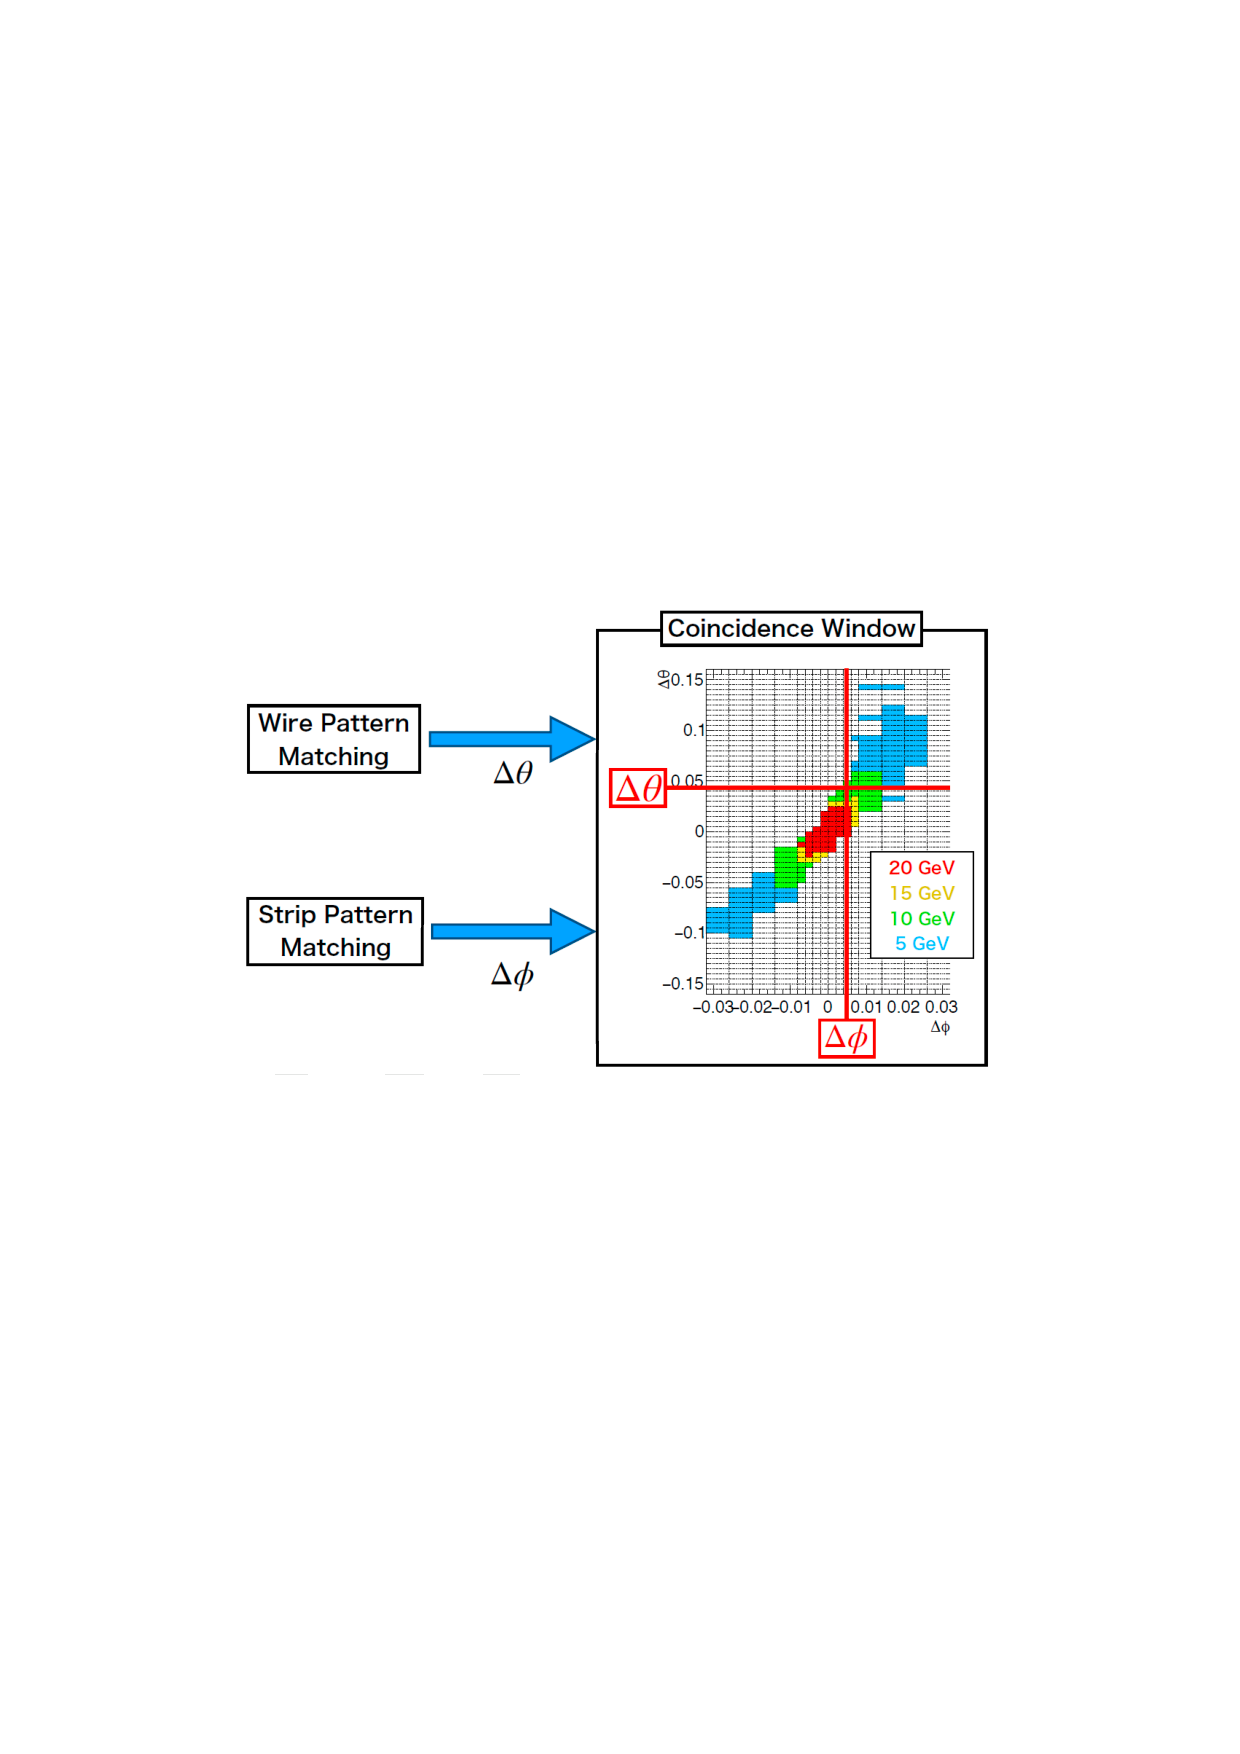
\includegraphics[width=16cm]{fig/SL/Concept_WS.pdf}
\caption[Wire Strip CoincidenceにおけるCoincidence Windowの例]{Wire Strip CoincidenceにおけるCoincidence Windowの例\cite{SLPDR}。本番運用時には$p_\mathrm{T}$は4 bit、16段階で出力する予定であるが、現状はテストのため5 GeV、10 GeV、15 GeV、20 GeVの4段階で出力している。}
\label{Concept_WS}
\end{figure}

\subsubsection*{Wire Strip CoincidenceのHDL実装}
駆動クロックはLHCバンチ交差クロックに同期した160 MHzクロック。レイテンシーは6クロックチック分 (37.5 ns)である。
Wire Strip CoincidenceではReginoと呼ばれる単位領域を新たに設定し、Regionごとに並列にコインシデンスを行う。Regionは後段のInner Coincidenceのコインシデンスをとる単位に合わせて定義されている。Wire Strip CoincidenceにおけるRegionの定義を図\ref{WS_region}に示す。エンドキャップ領域は|$\eta$| < 1.3 領域では 8 Unit、|$\eta$| < 1.3 領域では32 Unit という異なる大きさの Regionを定義し、それぞれの領域を22分割、13分割する。フォワード領域は32 Unit Regionで8分割する。

\begin{figure} 
\centering
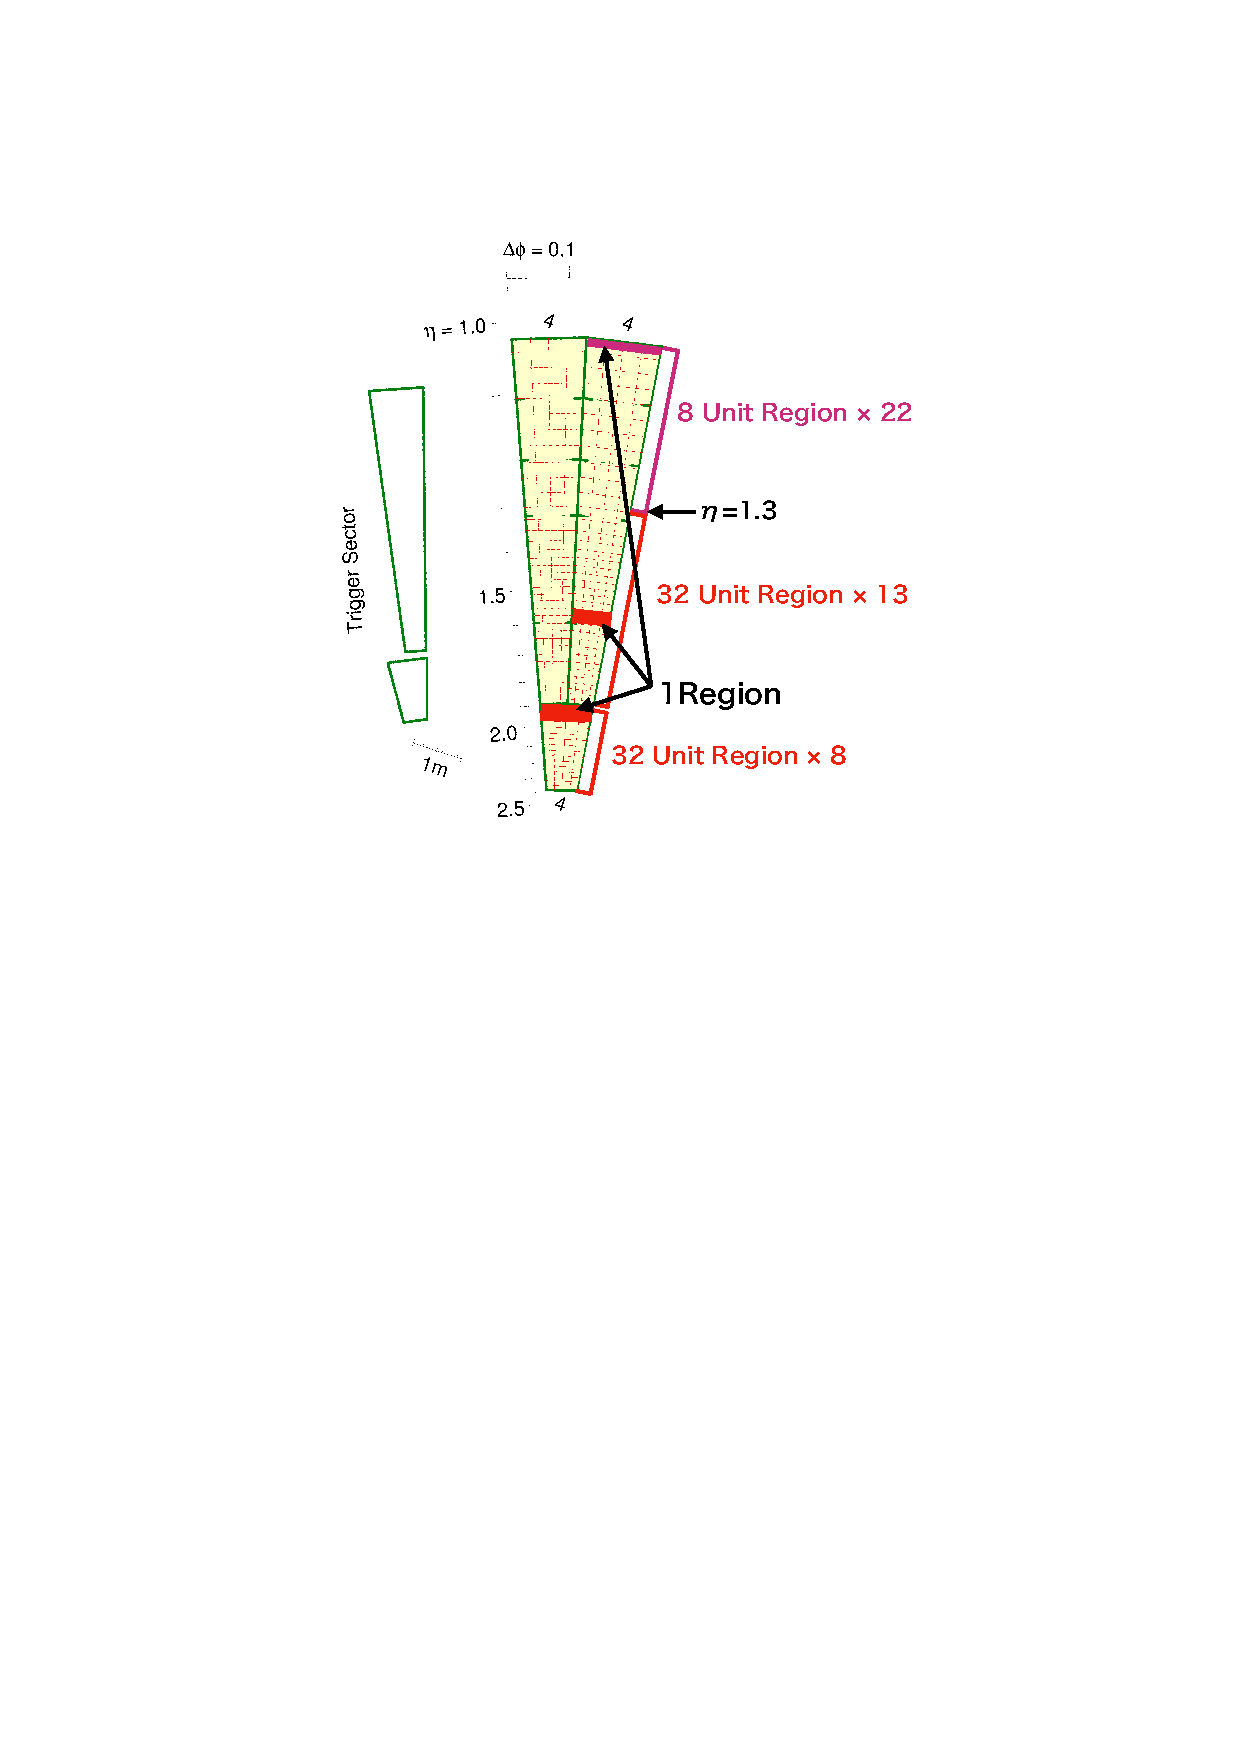
\includegraphics[width=16cm]{fig/SL/WS_region.pdf}
\caption[Wire Strip Coincidence以降のRegionの分割]{Wire Strip Coincidence以降のRegionの分割\cite{mt_kawamoto}。Endcap 領域では 8 Unit Regionと32 Unit Regionという2種類の領域を用意する。}
\label{WS_region}
\end{figure}

図\ref{WS_Concept}に1つのUnitの構造を示す。8 Unit Regionはトリガーセクターの全て$\phi$領域に当たるストリップの4 Unitからのstrip segmentと ワイヤーの2 Subunitからのwire segmentを組み合わせて、最大1つの飛跡候補を出力する。32 Unit Regionはストリップの 4 Unitからのstrip segmentと、ワイヤーの 8 Subunitからのwire segmentを組み合わせて、最大4つの候補を出力する。SL全体では最大180この飛跡候補が出力される。

\begin{figure} 
\centering
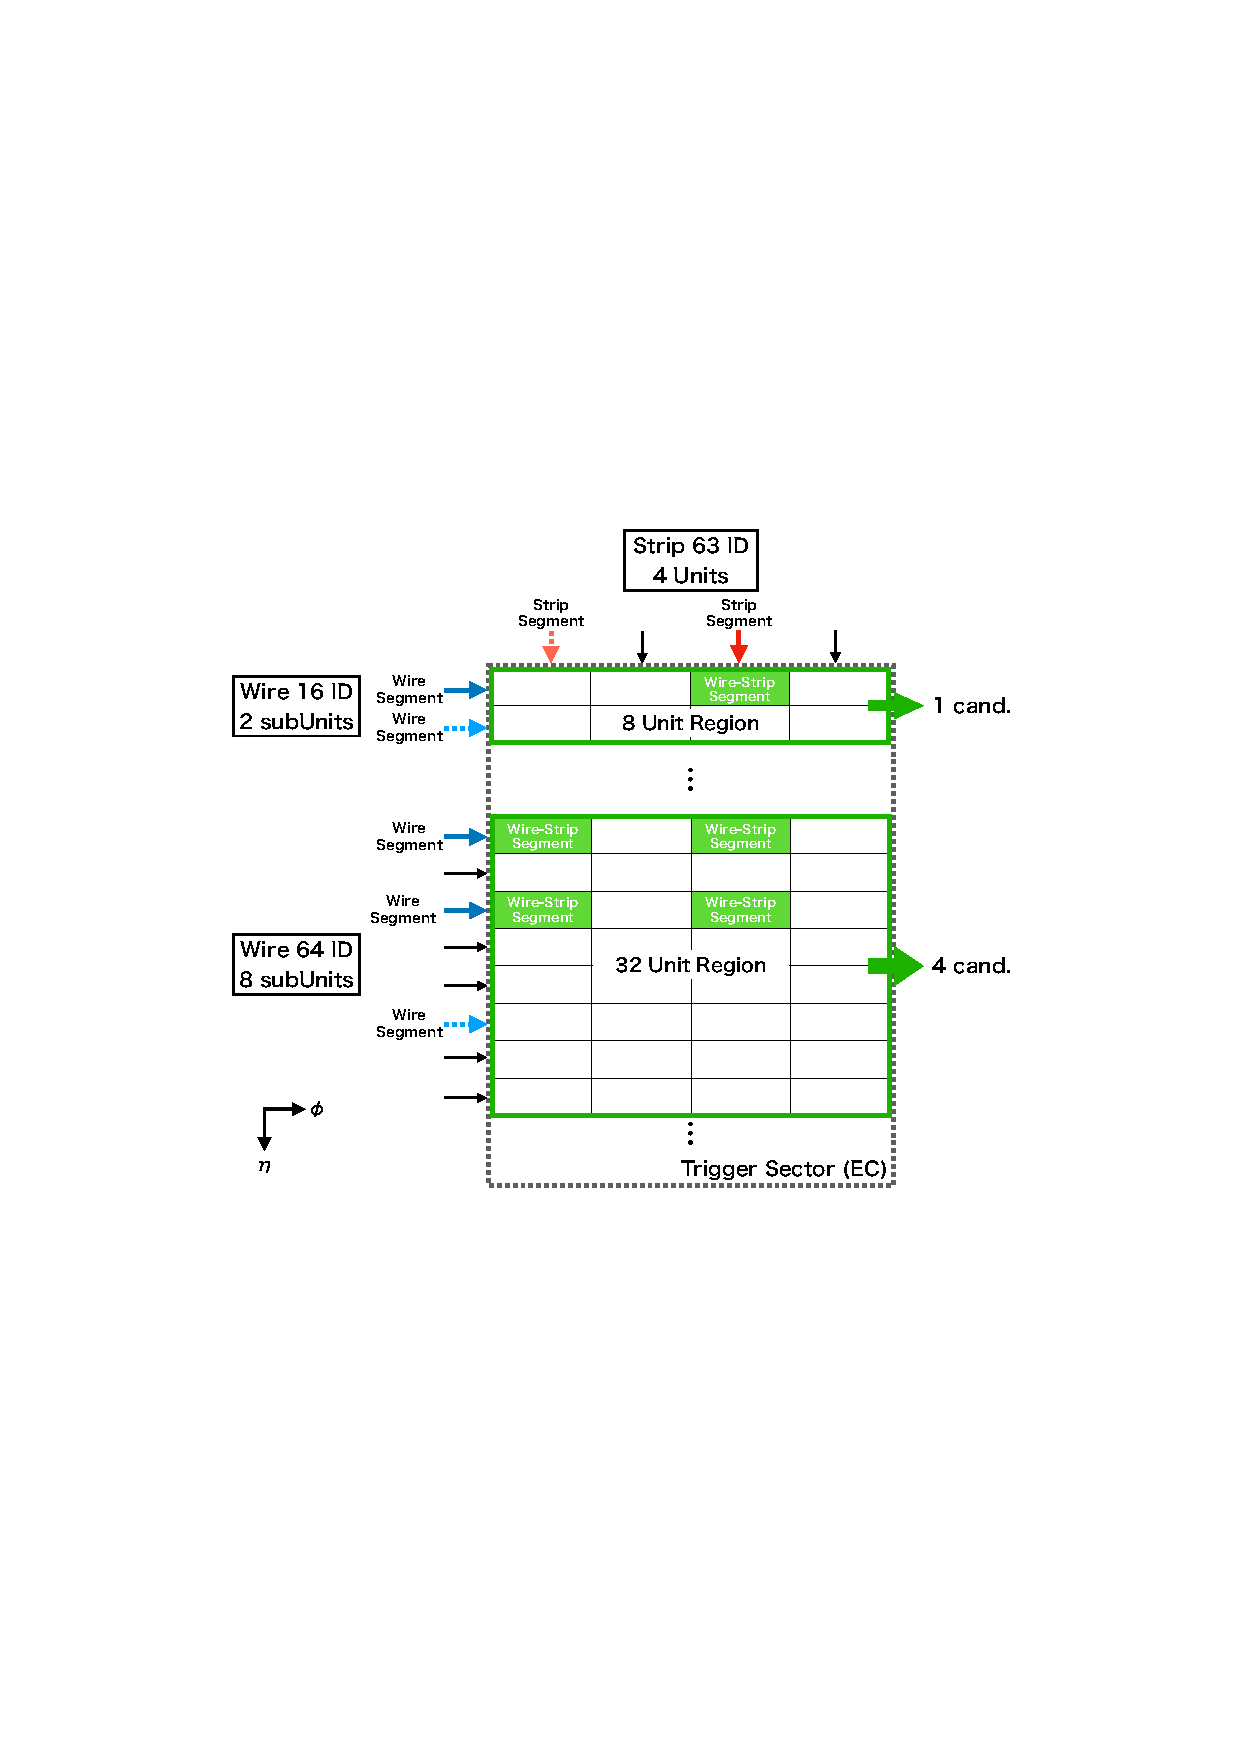
\includegraphics[width=16cm]{fig/SL/WS_Concept.pdf}
\caption[]{8 Unit Region、32 Unit Regionにおけるコインシデンスの概要\cite{mt_kawamoto}}
\label{WS_Concept}
\end{figure}

Wire Strip Coincidenceの各Unit内でのロジックの概要を図\ref{}に示す。各ユニットは\pt Calculator、Wire Position Corrector、Block Selectorで構成される。以下でそれぞれのモジュールについて述べる。

\begin{figure} 
\centering
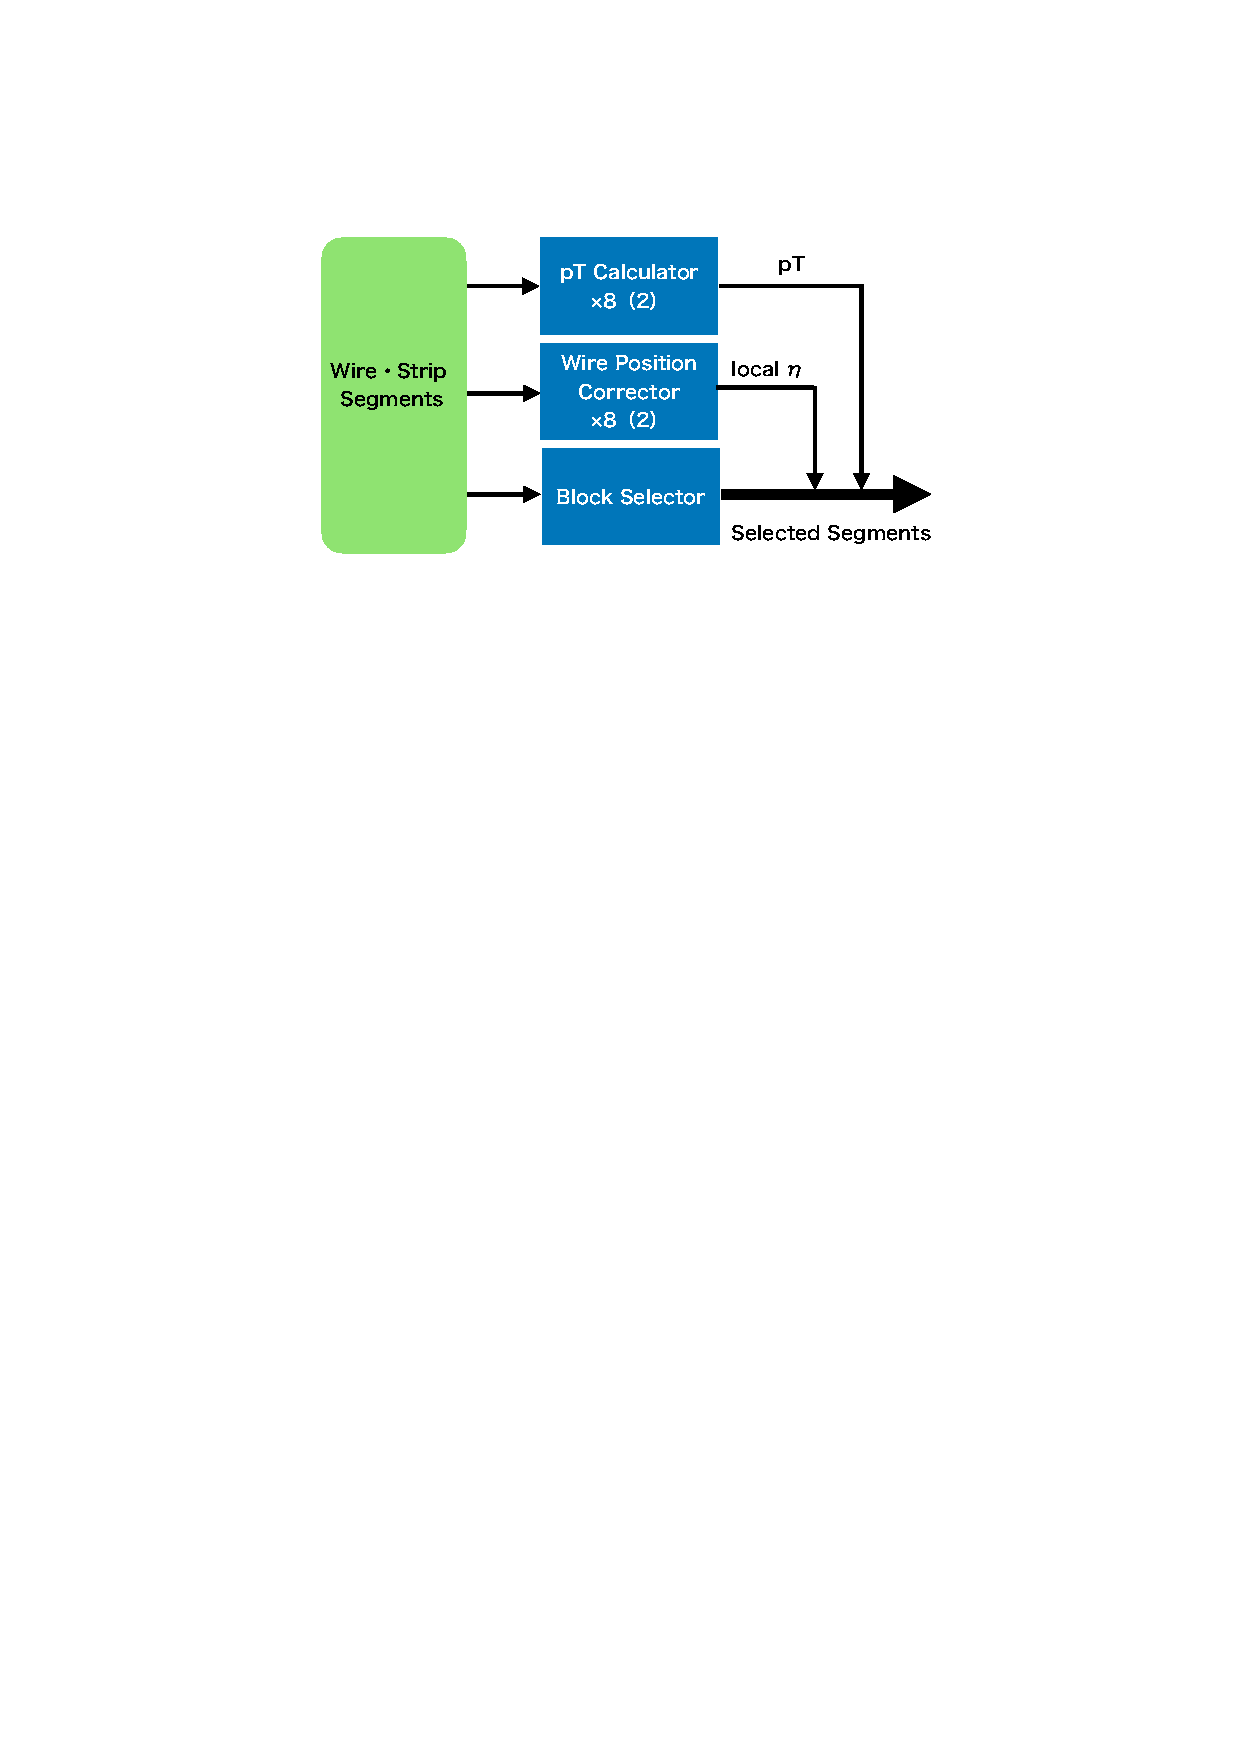
\includegraphics[width=16cm]{fig/SL/WS_logic.pdf}
\caption[Wire Strip Coincidence ファームウェアの概要]{Wire Strip Coincidence ファームウェアの概要\cite{mt_kawamoto}}
\label{WS_logic}
\end{figure}

\subsubsection*{\pt Calculator}
\pt Calculatorはwire segmentに含まれる8 bitの$\Delta\theta$及びstrip segmentに含まれる9 bitの$\Delta\phi$から、Coincidence Windowにアクセスするためのアドレスを作成し、Coincidence Windowに格納された4 bitの\pt を出力する。1つの\pt Calculatorは1つのwire segmentと4つのstrip segmentを組み合わせ、全ての組み合わせに対して\pt を出力する。Coincidence WindowはFPGAのdual BRAM上に格納されているため、この処理は2クロックチックで完了する。

\subsubsection*{Wire Position Corrector}
wire segment や strip segmentに含まれる位置情報は代表点のIDだが、Inner Coincidenceでは位置情報として$\eta$を利用する。また、代表点IDと$\eta$の関係はUnit Regionごとにばらつきがあることが知られており\footnote{wireの代表点が$\eta$に対して均一に並んでいないことと、$\phi$位置ごとでも代表点と$\eta$の対応関係は異なることによる}、全てのUnitで共通に変換できる訳ではない。そこでwireとstripの代表点と$\eta$位置の対応関係をパターンリストとして保存し、Unitごとに$\eta$の再構成を行う。これを担当するモジュールWire Position Correctorと呼ぶ。

\subsubsection*{Block Selector}
Block Selectorはワイヤーとストリップの組み合わせで生じる複数のミューオン飛跡候補から、後段に送る飛跡候補を選択する。飛跡の選抜はマッチした層数の多さを基準に行い、マッチした層数も同じ場合は角度がより小さいものを選択する。8 Unit Regionでは4つのストリップ飛跡と2つのワイヤー飛跡から再構成される計8個の飛跡候補から、最大1つの候補を絞り込む。32 Unit Regionでは4つのストリップ飛跡と8つのワイヤー飛跡の組み合わせからなる32個の飛跡候補から最大4つの候補を選ぶ。この時、2つは$\Delta\theta$が正の方向に曲げられたもの,もう2つは負に曲げられたものが選ばれるように設計する。これはJ/$\psi$ 粒子などから生じる、2つの異符号ミューオンを積極的に取れるようにするための実装である。
Wire Strip CoincidenceからInner Coincidenceに送られる飛跡情報のフォーマットを図\ref{tab:WS}に示す。本研究ではChannel MappingからWire Strip CoincidenceまでのトリガーロジックをTGC BW Coincidenceと呼ぶ。

\begin{table}[]
    \centering
    \caption{Wire Strip Coincidenceにおける飛跡候補のデータフォーマット}
    \label{tab:WS}
    \begin{tabular}{|c|c|}
    \hline
    \# of bits & Name                                                                                        \\ \hline\hline
    1          & Valid flag which means this region receive the more than one strip segment and wire segment \\ \hline
    4          & $p_{\mathrm{T}}$ threshold reconstructed using Coincidence Window                           \\ \hline
    8          & Local $\eta$ position in the unit                                                           \\ \hline
    3          & Unit ID                                                                                     \\ \hline
    7          & Angle difference $\Delta\eta$ between the segment and the vector from IP                    \\ \hline
    2          & Number of stations with the hits used for wire segment reconstruction                       \\ \hline
    4          & Angle difference $\Delta\phi$ between the segment and the vector from IP                    \\ \hline
    2          & Number of stations with the hits used for strip segment reconstruction                      \\ \hline
    \end{tabular}
\end{table}

\subsection{Inner Coincidence}
\subsubsection*{コンセプト}
nner CoincidenceではTGC BW コインシデンスで再構成された飛跡候補と磁場領域内部の検出器 (NSW、RPC BIS78、TGC EI、Tile カロリメーター)でコインシデンスととることで、衝突点に由来しないフェイクトリガーの削減と\pt 分解能の向上を図る。磁場内部に位置する検出器はそれぞれ異なる特徴を持っているため、コインシデンスをとる検出器ごとに独立したロジックが用意されている。ここでは具体例としてNSWとのコインシデンスロジックについて説明する。

図\ref{Concept_NSW}にNSWとのコインシデンスアルゴリズムの概要を示す。衝突点から飛来するミューオンはNSWにヒットを残した後エンドキャップトロイド磁場により主に$\eta$方向に曲げられ、TGCにヒットを残す。そのためTGC BW コインシデンスで再構成された$\eta$位置($\eta_{\mathrm{TGC}}$)とNSWで再構成された$\eta$位置($\eta_{\mathrm{NSW}}$)差が\pt と相関をもつ。この差$d\eta$を式(\ref{eq:deta})に定義する。

\begin{figure} 
\centering
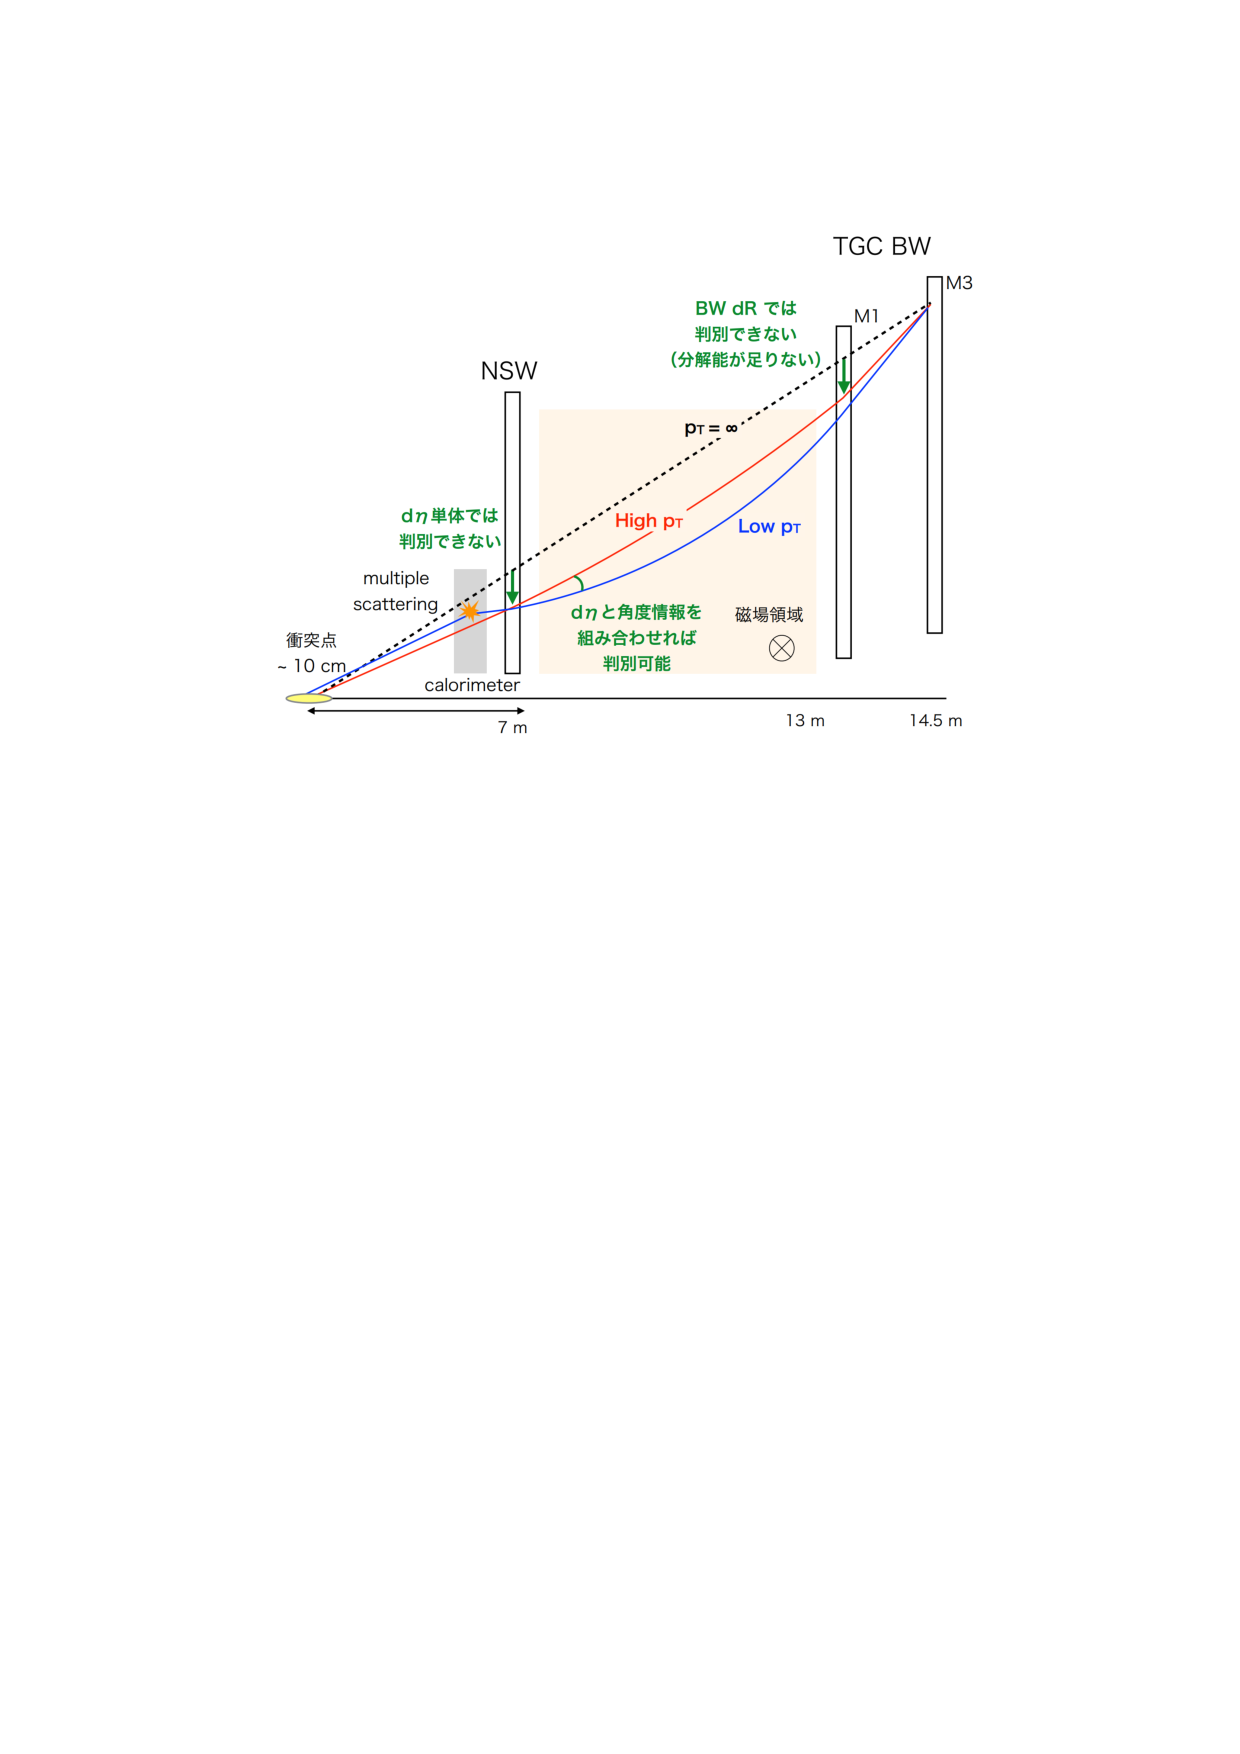
\includegraphics[width=16cm]{fig/SL/Concept_NSW.pdf}
\caption[NSW を用いたコインシデンスロジックの概要]{NSW を用いたコインシデンスロジックの概要\cite{mt_akatsuka}}
\label{Concept_NSW}
\end{figure}

\begin{equation}
    d\eta = \eta_{\mathrm{TGC}} - \eta_{\mathrm{NSW}}
    \label{eq:deta}
\end{equation}

しかし、衝突点から飛来するミューオンは検出器内部の物質 ( 主に物質量の大きいカロリーメータ )と多重散乱を起こすことがあり、この場合では$d\eta$のみでは\pt が高いものと低いものを見分けることができない。そこで、ミューオンがNSWに入射した角度 ($\Delta\theta_{\mathrm{NSW}}$) を分別変数として追加することで、より正確に\pt 判定を行うことができる。この計算にも$d\eta$、($\Delta\theta_{\mathrm{NSW}}$) を入力、\pt を出力としたCoincidence Windowが利用される。

\subsubsection*{Inner CoincidenceのHDL実装}
このモジュールの駆動クロックは、LHC クロックに同期した周波数 160 MHz のクロックであり、レイテンシーは 7 クロックチック分 (43.75 ns) である。

Inner CoincidenceもRegionを1単位として並列に処理が行われる。$\eta$位置ごとにどの検出器とコインシデンスをとるかが決められており、|$\eta$| < 1.3 の領域では主にRPC、EI、Tileカロリメーターと、|$\eta$| > 1.3の領域では主にNSWとコインシデンスをとる。8 Unit RegionはWire Strip Coincidenceから1つの飛跡候補を受け取り、コインシデンスをとった後1候補を出力する。32 Unit RegionはWire Strip Coincidenceから4つの飛跡候補を受け取り、2つまで候補を絞って出力する。その結果SL全体では最大112候補を出力する。

Inner Coincidenceの各Unit 内でのロジックの概要を図\ref{Inner_logic}に示す。各ユニットはDecoder、Coincidence、Which Innerで構成される。以下に例としてNSWとのコインシデンスをとるRegionについて説明する。

\begin{figure} 
\centering
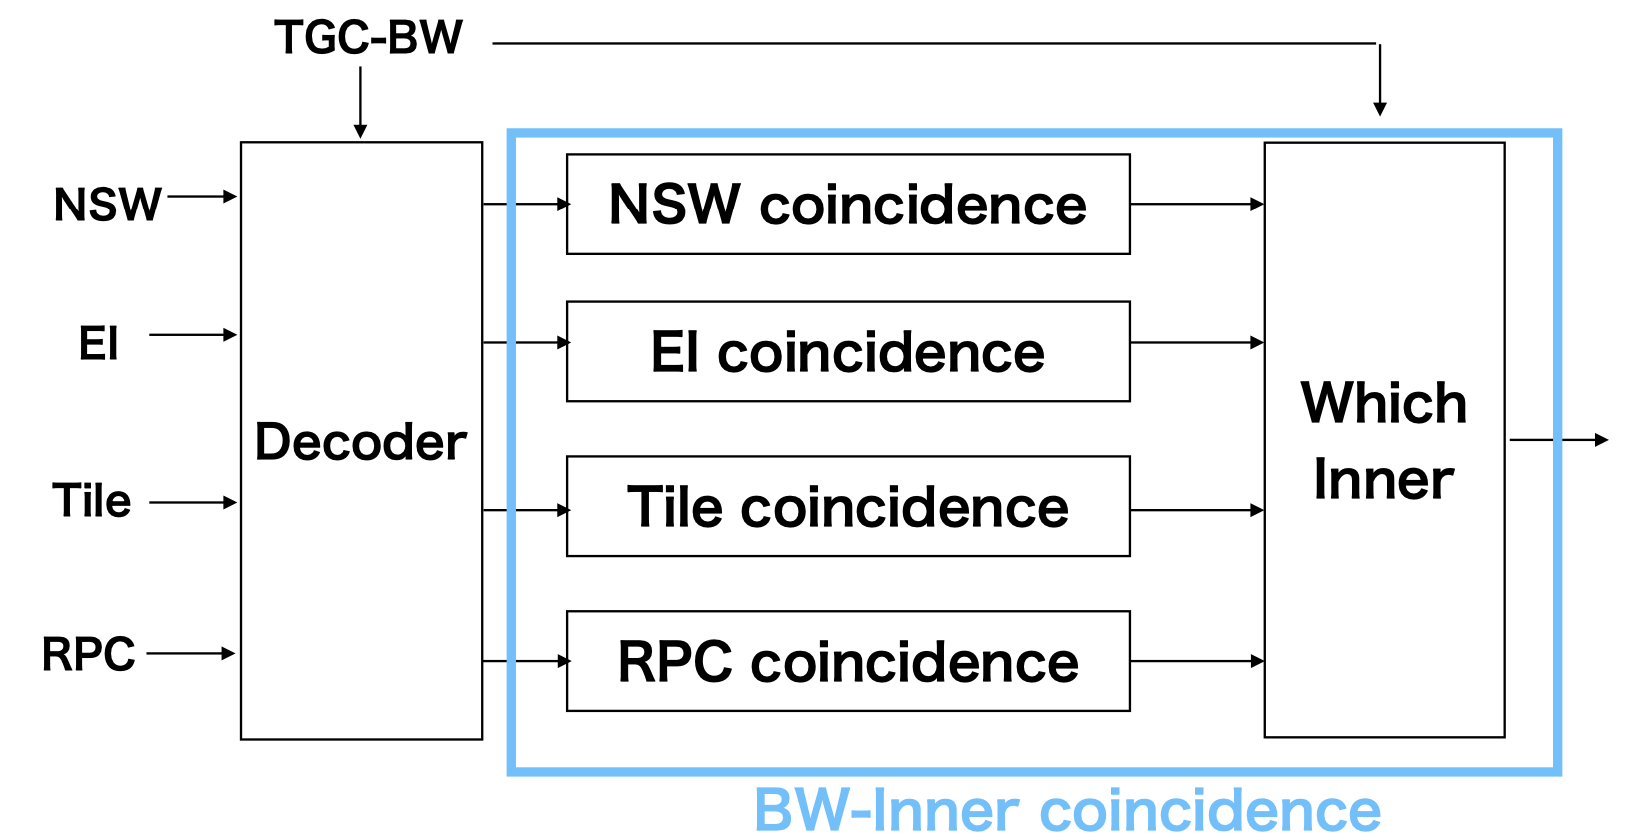
\includegraphics[width=16cm]{fig/SL/Inner_integrate.png}
\caption[Inner Coincidenceの概要]{Inner Coincidenceの概要\cite{mt_kobayashi}}
\label{Inner_logic}
\end{figure}

\begin{itemize}
    \item Decoder\\
    1つのSLはNSWで再構成された飛跡を最大16個受け取る。この中からTGC BW コインシデンスで再構成された飛跡候補と組み合わせる4候補を選ぶのがDecoderである。ここでは\pt が大きいミューオンの検出効率を高く保つため、|$d\eta$|が小さいものを優先的に選別する。
    \item NSW Coincidence\\
    TGC BW の1つの飛跡候補とNSWの4つの飛跡候補でコインシデンスをとる。Coincidence WindowはFPGAのURAMに格納されており、8 bitの$d\eta$情報と4 bitの$\Delta\theta$を入力、4 bitの\pt を出力とする。計算された飛跡のうち、\pt が最大の候補が保存され40 MHzごとに出力される。
    \item Which Inner\\
    Which Inner モジュールは複数の検出器とのコインシデンスロジックが並列に走る|$\eta$| < 1.3の領域において、どの検出器とのコインシデンス結果を最終出力とするかを決定する。
\end{itemize}

Inner CoincidenceからTrack Selectorに送られる飛跡候補のデータフォーマットを表 \ref{tab:InnerCoin} に示す。

\begin{table}[]
    \centering
    \caption{Inner Coincidenceにおける飛跡候補のデータフォーマット}
    \label{tab:InnerCoin}
    \begin{tabular}{|c|c|c|}
    \hline
    \# of bits & Name                             & Comment                                                                \\ \hline\hline
    14         & TGC $\eta$                       & $\eta$ in global candidate at the pivot plane of TGC                   \\ \hline
    9          & TGC $\phi$                       & $\phi$ in global candidate at the pivot plane of TGC                   \\ \hline
    8          & TGC \textbackslash{}pt           & TGC transverse momentum                                                \\ \hline
    4          & TGC \textbackslash{}pt threshold & TGChighest \textbackslash{}pt thresholdsatisfied                       \\ \hline
    1          & TGC charge                       & TGC TC charge                                                          \\ \hline
    3          & Coincidence type                 & Identifier of coincidence type                                         \\ \hline
    14         & MDT $\eta$                       & $\eta$ coordinate of the MDT segment position of the innermost station \\ \hline
    8          & MDT \textbackslash{}pt           & MDT transverse momentum                                                \\ \hline
    4          & MDT \textbackslash{}pt threshold & MDThighesttransversemomentumthresholdsatisfied                         \\ \hline
    1          & MDT charge                       & MDT charge                                                             \\ \hline
    4          & MDT Processing Flag              & Type of reconstructed muon                                             \\ \hline
    2          & \# of segments                   & Number of MDT segments associated to the muon                          \\ \hline
    3          & Segment quality flag             & Quality of each segment                                                \\ \hline
    49         & Reserved                         &                                                                        \\ \hline
    \end{tabular}
\end{table}

\subsection{Track Selector}
\subsubsection*{コンセプト}
Track SelectorはInner Coincidenceから出力される最大112個のミューオン飛跡候補からMUCTPIに送る6候補を選ぶ。このときInner Coincidenceで判定された\pt が高いものを優先的に選択する。

\subsubsection*{Track SelectorのHDL実装}
モジュールの駆動クロックはLHCクロックに同期した周波数160 MHzのクロックであり、レイテンシ-は5クロックチック (31.25 ns)である。
概要を図\ref{TrackSelector_overview}に示す。候補選別回路は4 bitの\pt が大きい順に候補を並び替えるソーティングロジックとして実装される。特にBatcherの奇遇マージソート法\cite{Batcher}という、並列処理のもとで高速でソーティングを行うことができる手法が採用された。Track Selectorは16個の8-key sorting network、と15個の16-key merging networkで構成され、インプットが128、アウトプットが8のソーティングロジックとなっている。8-key soting networkおよび16-key merging networkの概要を図\ref{Sortiing_8key}、\ref{Sorting_16}に示す。これらの図の横線はワイヤーを示し、縦軸がコンパレーターを表す。左から右に1つの飛跡候補同士の比較が行われ、それの集合体としてロジックが実装される。


\begin{figure} 
    \centering
    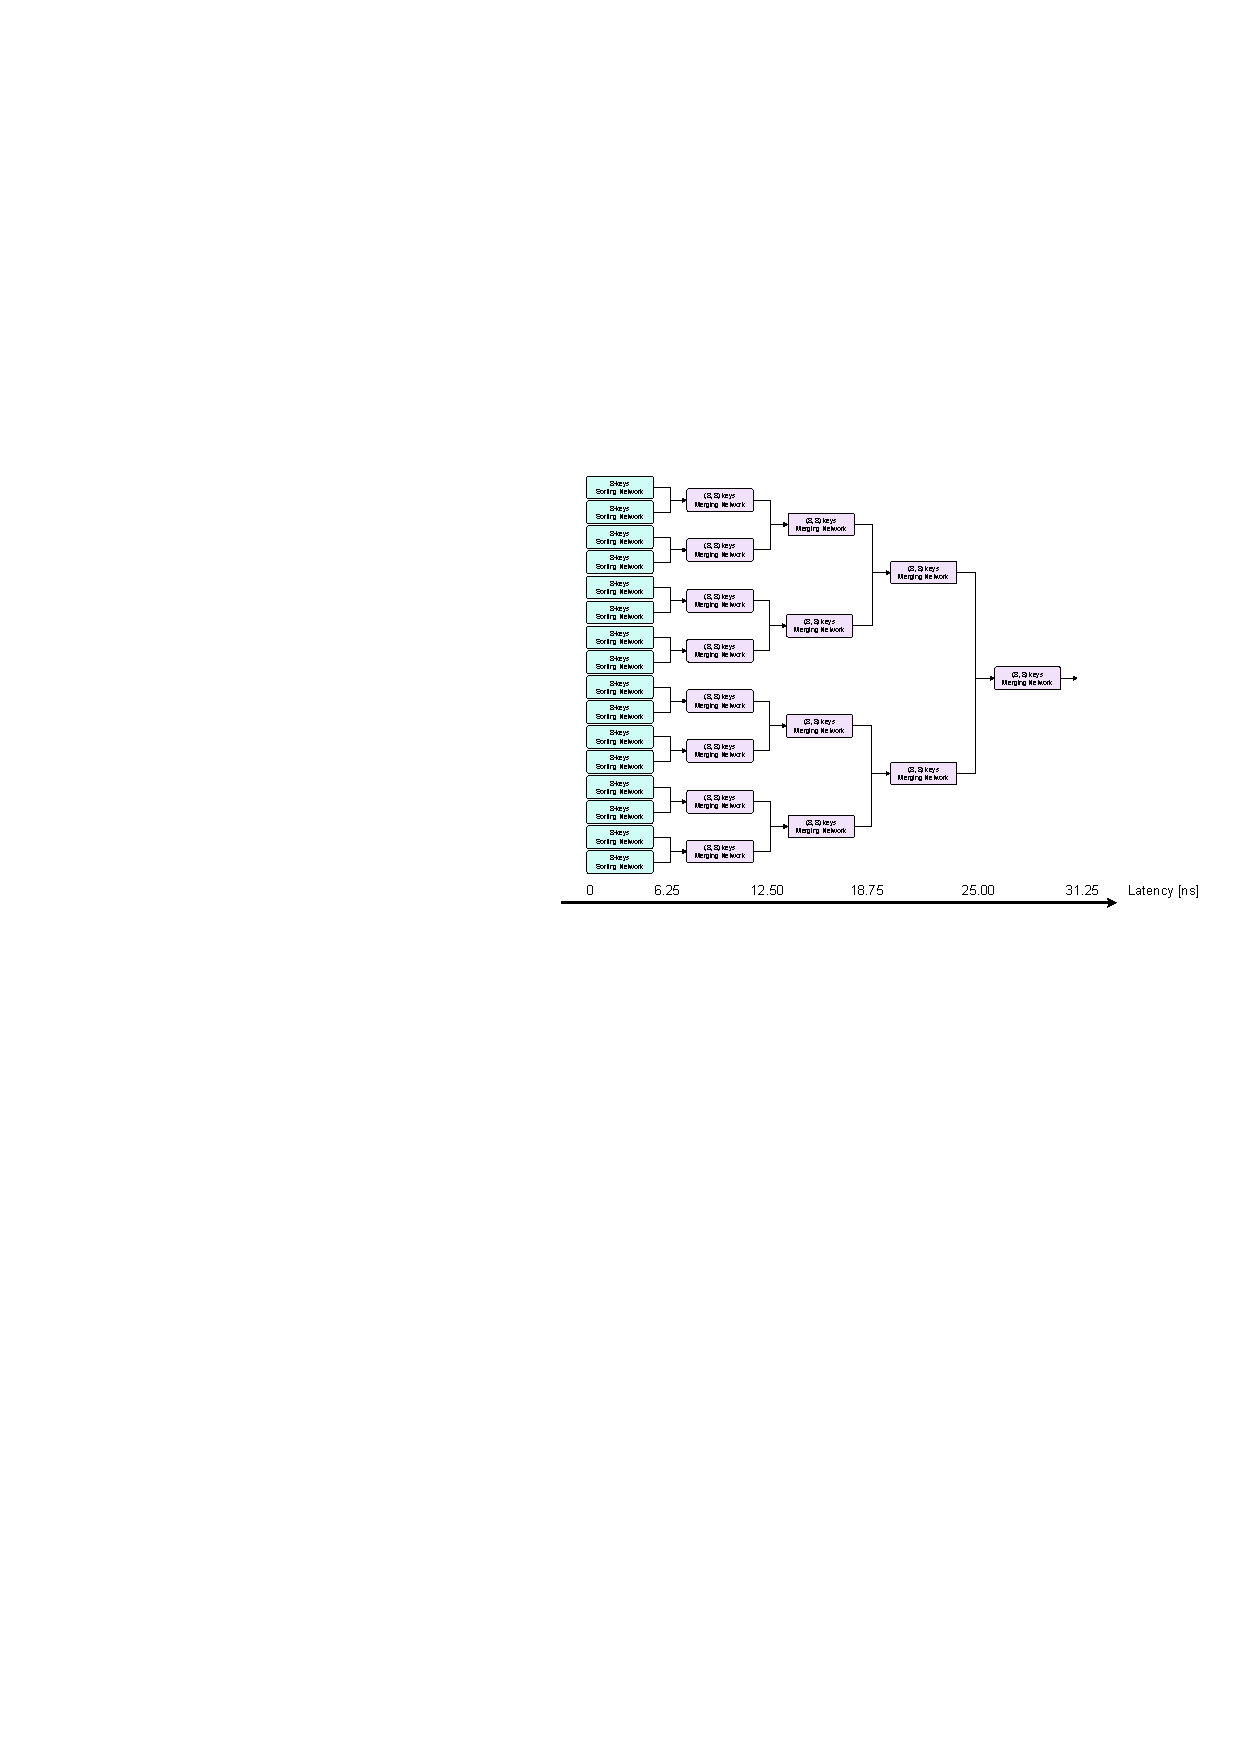
\includegraphics[width=16cm]{fig/SL/TrackSelector_overview.pdf}
    \caption[Track Selector の概要]{Track Selector の概要}
    \label{TrackSelector_overview}  
\end{figure}
    

\begin{figure} 
\centering
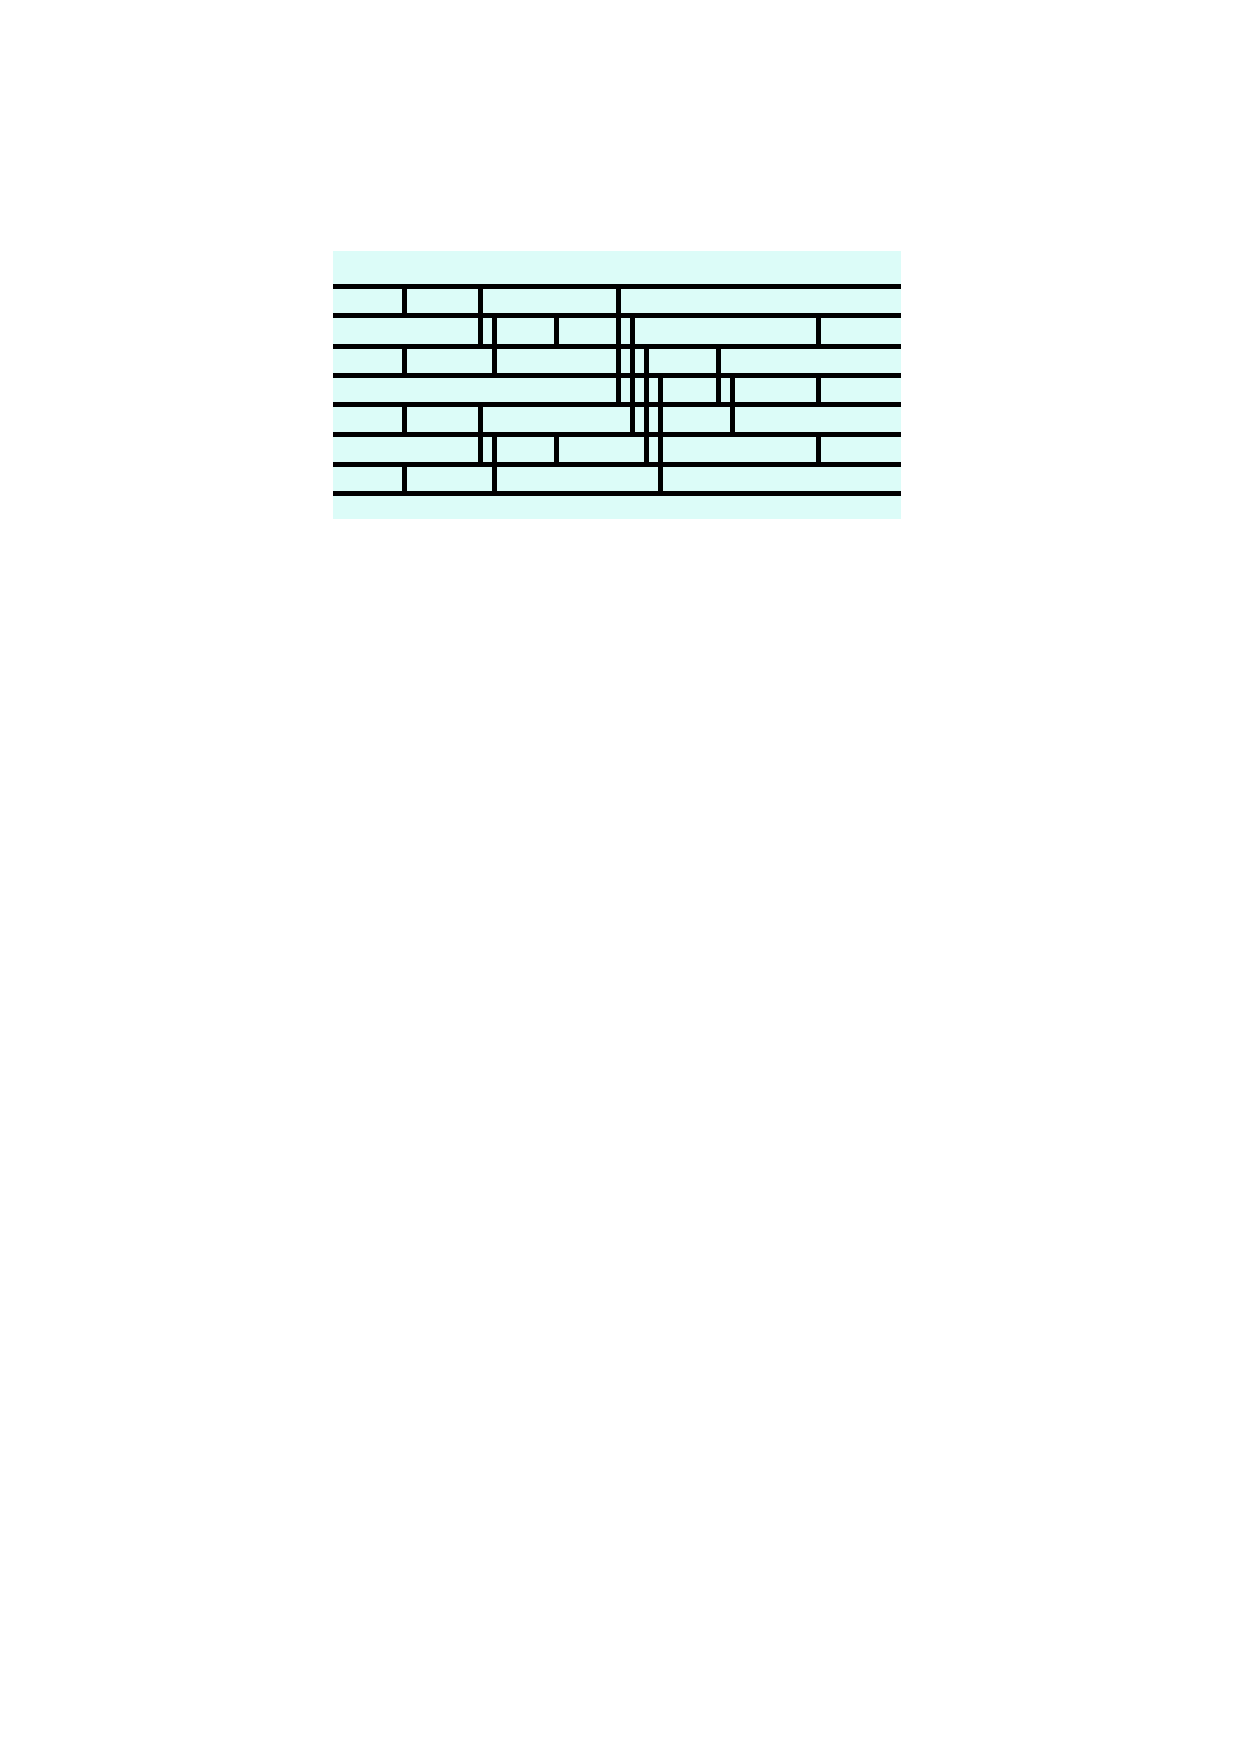
\includegraphics[width=16cm]{fig/SL/Sortiing_8key.pdf}
\caption[8-key sorting network の概要]{8-key sorting network の概要}
\label{Sortiing_8key}
\end{figure}

\begin{figure} 
\centering
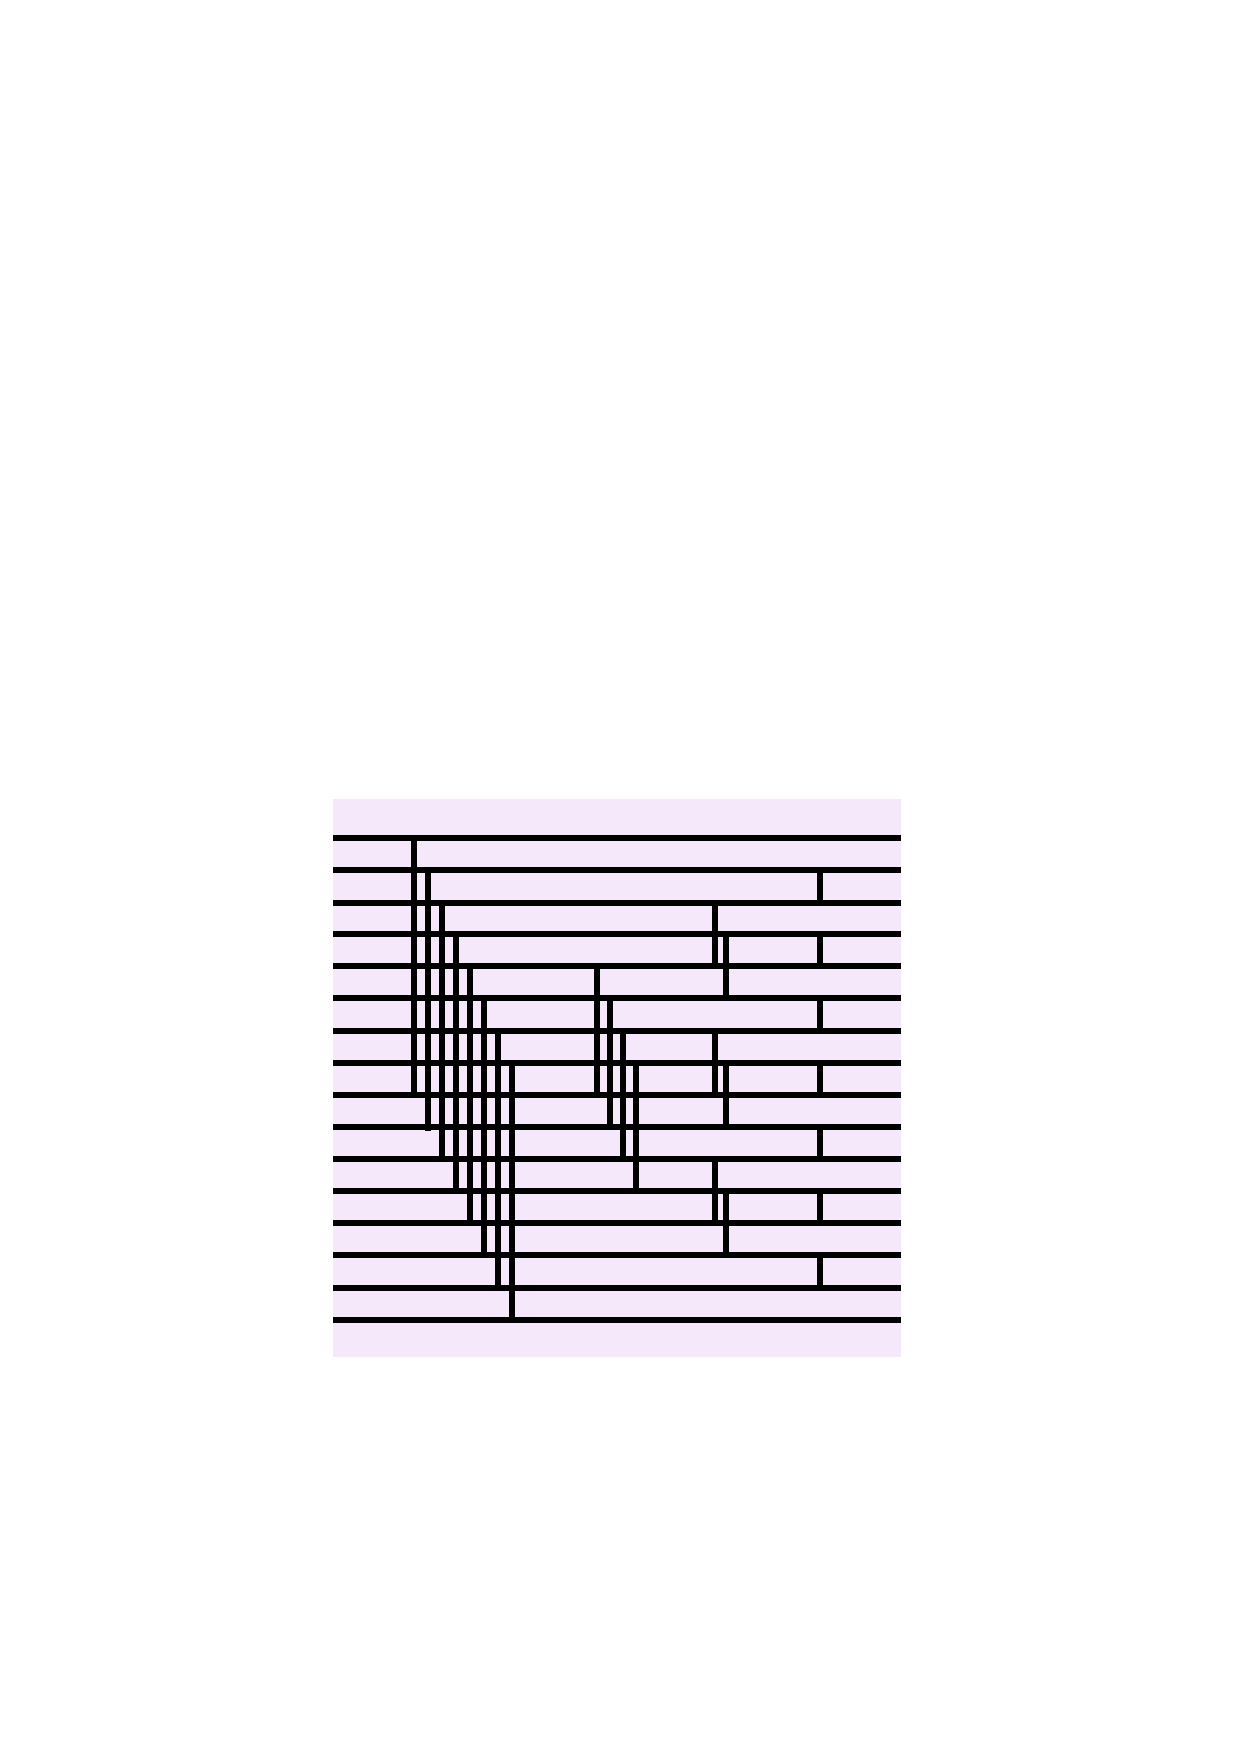
\includegraphics[width=16cm]{fig/SL/Sorting_16.pdf}
\caption[16-key merging network の概要]{16-key merging network の概要}
\label{Sorting_16}
\end{figure}


\newpage
\section{Inner Coincidenceの統合}
\label{sec_TriggerIntegration}
2章で述べたように、SL FPGAの中でトリガーロジックは図\ref{}のように統合される。
PS board とのインターフェイスが実装されるSLR0・2・3には、TGC BW Coincidenceが実装される。トリガーセクターごとにSLRが分けられ、SLR0にEndcap $\phi\,0$、SLR2にEndcap $\phi\,1$、SLR3にForwardのロジックが配置される。磁場内部の検出器やMUCTPIとのインターフェイスはSLR1に実装され、ここにはInner Coincidence、Track Selectorが配置される。
高輝度LHC-ATLAS実験に向けたトリガー開発は、これまでに各モジュールのHDL実装が完了し、Segment Reconstructionまでの統合が完了している。

本研究では引き続きWire Strip Coincidence、Inner Coincidence、Track Selectorの統合を進め、一連のトリガーロジックの統合を完了させる。以下にそれぞれの実装について述べる。

\subsection{Wire Strip Coincidenceの統合}
Wire Strip Coincidenceを統合ファームウェアに組み込むため、前段のWire Segment Reconstruction、Strip Segment Reconstructionの出力を配線した他、モジュール内に存在する2種類のLUTをコンフィギュレーションするパスを接続した。
Wire Strip Coincidenceモジュールに接続した各信号線を表\ref{tab:WS_integrate}にまとめる。

\begin{table}[]
    \centering
    \caption{Wire Strip Coincidenceにおける信号線}
    \label{tab:WS_integrate}
    \begin{tabular}{|c|c|}
    \hline
    接続するモジュール                               & 信号線 ( bit幅 )                                                                                                    \\ \hline
    Wire Segment Reconstruction             & \begin{tabular}[c]{@{}c@{}}Wire Segment ( EC : 148 subunit x 20 bit, \\ FW : 64 subunit x 20 bit )\end{tabular} \\ \hline\hline
    Strip Segment Reconstruction            & Strip Segment ( EC :  20 unit x 17bit, FW : 5 unit x 17 bit)                                                    \\ \hline
    LUT Manager for \textbackslash{}pt LUT  & Address + Data  (EC : 35 region x 18 bit、FW : 8 unit x 18 bit )                                                 \\ \hline
    LUT Manager for \textbackslash{}eta LUT & Address + Data (EC : 35 region x  17 bit、FW : 8 unit x 17 bit )                                                 \\ \hline
    \end{tabular}
\end{table}

Wire Strip CoincidenceはWire Segment Reconstructionの1つのサブユニットから1つの飛跡情報を受け取る。1つの飛跡情報は20 bitで構成され、8 bitの$\Delta\theta$、10 bitのM3代表点ID、2 bitのマッチレイヤーの情報が含まれる。Endcap領域には合計148のサブユニットが存在するため、合計2960 bit、Foward領域では64のサブユニットが存在するため、合計1280 bitの信号線を接続した。
Strip Segment Reconstructionからは1つのユニットから1つの飛跡情報を受け取る。1つの飛跡情報は17 bitで構成され、9 bitの$\Delta\phi$、6 bitのM3代表点ID、2 bitのマッチレイヤー情報が含まれる。Endcap領域には計20のユニットが存在するため、合計340 bit、Foward領域では5つのニットが存在するため、合計 85 bitの信号線を接続した。

Wire Strip Coincidence モジュール内に配置されている\pt 出力用のBRAMと$\eta$ 出力用のBRAMのコンフィギュレーションはMPSoCから行う。MPSoCからの書き込みを仲介するためのモジュールとしてWire Strip Coincidence用のLUT Managerを実装した。MPSoC から各モジュールのLUT ManagerまではRAM ID、Data、address、Write enableという共通の信号線を接続する。LUT ManagerはRAM IDをモニターし、担当するモジュールに該当するRAM IDが指定されたときのみ、addressとData信号をラッチしてRAMに書き込み動作を行う。これによりMPSoCから各RAMに個別の配線を用意する必要がなく、統一的に書き込み動作を実行することができる。また、モジュール内のBRAMはLHCバンチ交差クロックを逓倍した160 MHzクロックで動作するが、LUTの書き込みはMPSoCからのスローなコントロールに使用される50 MHzクロックで行う。この二つはソースが異なるクロックであるため、ここにはクロックドメインをまたぐための仕掛けもに実装してある。

\subsection{Inner Coincidenceの統合}
Inner Coincidenceを実機上で稼働させるために、Wire Strip Coincidenceの出力、磁場内部の検出器からの飛跡情報、LUTのコンフィギュレーションパスを実装した。Inner Coincidence モジュールに接続した各信号線を表\ref{tab:Inner_integrate}にまとめる。

\begin{table}[]
    \centering
    \caption{Inner Coincidenceにおける信号線}
    \label{tab:Inner_integrate}

    \begin{tabular}{|c|c|}
    \hline
    接続するモジュール                                & 信号線 ( bit幅 )                                                                                                                   \\ \hline\hline
    Wire Strip Coincidence SLR0              & \begin{tabular}[c]{@{}c@{}}8 region (31 bit x 1 cand x 22 regions) \\ + 32 region (31 bit x 4 cand x 13 regions )\end{tabular} \\ \hline
    Wire Strip Coincidence SLR2              & \begin{tabular}[c]{@{}c@{}}8 region (31 bit x 1 cand x 22 regions) \\ + 32 region (31 bit x 4 cand x 13 regions )\end{tabular} \\ \hline
    Wire Strip Coincidence SLR3              & 32 region (31 bit x 4 cand x 8 regions )                                                                                       \\ \hline
    LUT Manager for \textbackslash{}pt NSW   & Address + Data  (86 bit x 78 region )                                                                                          \\ \hline
    LUT Manager for \textbackslash{}eta RPC  & Address + Data (21 bit x 46 region )                                                                                           \\ \hline
    LUT Manager for \textbackslash{}pt EI    & Address + Data (15 bit x 46 region )                                                                                           \\ \hline
    LUT Manager for \textbackslash{}eta TIle & Address + Data (18 bit x 46 region )                                                                                           \\ \hline
    Test Register for NSW                    & 19 bit x 16 cand                                                                                                               \\ \hline
    Test Register for RPC                    & 24 bit x 4 cand                                                                                                                \\ \hline
    Test Register for EI                     & 22 bit x 4 cand                                                                                                                \\ \hline
    Test Register for Tile                   & 16 bit x 4 cand                                                                                                                \\ \hline
    \end{tabular}
\end{table}

Inner CoincidenceはWire Strip Coincidenceの8 Regionから1つ、32 Regionから4つの飛跡情報を受け取る。1つの飛跡情報は31 bitで構成され、1 bitのvalid信号、4 bitの\pt 閾値、8 bitの$\eta$ positionに加え、計17にリダクションしたWire SegmentおよびStrip Segmentが含まれる。そのため、Endcap領域を処理するSLR0、SLR2からそれぞれ4,650 bit、FW領域を処理するSLR3から992 bitの信号線をSLRを跨いで接続した。

Inner CoincidenceはNSW、EI、TIle、RPCからの位置情報や角度情報を入力として利用する。しかし、磁場内部の検出器から送られるデータの詳細が決まっておらず、それを受け取るためのインターフェイスも実装されていない。そこで、今回はMPSoCから書き込むことができる試験用のレジスタと接続した。各種へのコンフィギュレーションのため、Inner Coincidence用のLUT Managerを実装し、同様に配線した。

Inner Coincidenceは112このミューオン飛跡候補を出力し、1飛跡候補につき128 bitの情報を出力する。合計112 候補 x 128 bitの信号はTrack Selectorに接続した。Track Selectorから出力される6候補 x 128 bitの信号は、 MDTTPやMUCTPIへのインターフェイスは実装中であるため、MPSoCから読み出せる試験用のレジスタと配線した。

\subsection{トリガーロジック統合後のリソース使用量}

本研究により、トリガーロジックのすべてのモジュールがSL FPGAへ統合され、フルチェーンでのリソース使用量を見積もることができるようになった。
Inner Coincidenceを統合した後のデバイスのリソース使用状況を表\ref{tab:Resource_after1}に示す。表中の値は、1つのSLR中のリソースに対する使用量の割合を百分率で表したものである。Totalにはトリガーロジックだけでなく、コントロール、リードアウトのロジックも含めたリソース使用状況を示している。
また、現状、トリガーロジックはタイミング違反を起こすことなく実装を完了しているが、そのために幾つかの最適化を行った。この詳細はAppendix\ref{}で説明する。

\begin{table}[]
    \centering
    \caption{最適化後のデバイスのリソース使用状況}
    \label{tab:Resource_after1}
    \begin{tabular}{|c|c|c|c|c|c|c|c|}
    \hline
    Name                                                                        & Block                        & \begin{tabular}[c]{@{}c@{}}LUT \\ (17280000)\end{tabular} & \begin{tabular}[c]{@{}c@{}}REG \\ (34560000)\end{tabular} & \begin{tabular}[c]{@{}c@{}}CLB \\ (2160000)\end{tabular} & \begin{tabular}[c]{@{}c@{}}LUT \\as Memory \\ (791040)\end{tabular} & \begin{tabular}[c]{@{}c@{}}BRAM \\ (2688)\end{tabular} & \begin{tabular}[c]{@{}c@{}}URAM\\  (1280)\end{tabular} \\ \hline\hline
    \multirow{6}{*}{\begin{tabular}[c]{@{}c@{}}SLR0 \\ EC $\phi$1\end{tabular}} & Wire Station Coincidence     & 7.4                                                       & 1.48                                                      & 22.2                                                     & 0                                                                 & 0                                                      & 0                                                      \\ \cline{2-8} 
                                                                                & Strip Station Coincidence    & 0                                                         & 0.2                                                       & 0.84                                                     & 0                                                                 & 0                                                      & 0                                                      \\ \cline{2-8} 
                                                                                & Wire Segment Reconstruction  & 16.28                                                     & 4.44                                                      & 26.64                                                    & 0                                                                 & 0                                                      & 45.88                                                  \\ \cline{2-8} 
                                                                                & Strip Segment Reconstruction & 6.24                                                      & 3.08                                                      & 13.44                                                    & 0.08                                                              & 0                                                      & 2.43                                                   \\ \cline{2-8} 
                                                                                & Wire Strip Coincidence       & 2.4                                                       & 2.92                                                      & 10.68                                                    & 0                                                                 & 37.52                                                  & 0                                                      \\ \cline{2-8} 
                                                                                & Total                        & 57.2                                                      & 25.68                                                     & 91.76                                                    & 3.6                                                               & 74.4                                                   & 51.56                                                  \\ \hline\hline
    \multirow{3}{*}{SLR1}                                                       & Inner Coincidence            & 66.92                                                     & 18.88                                                     & 87                                                       & 3                                                                 & 28.88                                                  & 50                                                     \\ \cline{2-8} 
                                                                                & Track Selector               & 7.56                                                      & 2.8                                                       & 17.56                                                    & 0                                                                 & 0                                                      & 0                                                      \\ \cline{2-8} 
                                                                                & Total                        & 79.16                                                     & 26.52                                                     & 99.24                                                    & 4.88                                                              & 28.88                                                  & 50                                                     \\ \hline\hline
    \multirow{6}{*}{\begin{tabular}[c]{@{}c@{}}SLR2 \\ EC $\phi$1\end{tabular}} & Wire Station Coincidence     & 8.88                                                      & 1.48                                                      & 22.2                                                     & 0                                                                 & 0                                                      & 0                                                      \\ \cline{2-8} 
                                                                                & Strip Station Coincidence    & 0                                                         & 0.2                                                       & 0.92                                                     & 0                                                                 & 0                                                      & 0                                                      \\ \cline{2-8} 
                                                                                & Wire Segment Reconstruction  & 14.8                                                      & 4.44                                                      & 29.6                                                     & 0                                                                 & 0                                                      & 45.88                                                  \\ \cline{2-8} 
                                                                                & Strip Segment Reconstruction & 6.24                                                      & 3.08                                                      & 13.6                                                     & 0.08                                                              & 0                                                      & 2.43                                                   \\ \cline{2-8} 
                                                                                & Wire Strip Coincidence       & 2.44                                                      & 2.92                                                      & 11.28                                                    & 0                                                                 & 37.52                                                  & 0                                                      \\ \cline{2-8} 
                                                                                & Total                        & 58.64                                                     & 27.04                                                     & 93.25                                                    & 3.96                                                              & 80.2                                                   & 51.56                                                  \\ \hline\hline
    \multirow{6}{*}{\begin{tabular}[c]{@{}c@{}}SLR3 \\ FW\end{tabular}}         & Wire Station Coincidence     & 1.44                                                      & 0.64                                                      & 3.36                                                     & 0                                                                 & 0                                                      & 0                                                      \\ \cline{2-8} 
                                                                                & Strip Station Coincidence    & 0                                                         & 0.04                                                      & 0.12                                                     & 0                                                                 & 0                                                      & 0                                                      \\ \cline{2-8} 
                                                                                & Wire Segment Reconstruction  & 6.4                                                       & 1.28                                                      & 10.88                                                    & 0                                                                 & 0                                                      & 19.84                                                  \\ \cline{2-8} 
                                                                                & Strip Segment Reconstruction & 1.24                                                      & 0.6                                                       & 2.64                                                     & 0.04                                                              & 0                                                      & 1.24                                                   \\ \cline{2-8} 
                                                                                & Wire Strip Coincidence       & 1.48                                                      & 1.4                                                       & 4.4                                                      & 0                                                                 & 14.28                                                  & 0                                                      \\ \cline{2-8} 
                                                                                & Total                        & 25.36                                                     & 13.36                                                     & 50.12                                                    & 1.84                                                              & 33.24                                                  & 20.32                                                  \\ \hline
    \end{tabular}
\end{table}